%%%%%%%%%%%%%%%%%%%%%%%%%%%%%%%%%%%%%%%%%
% Short Sectioned Assignment LaTeX Template Version 1.0 (5/5/12)
% This template has been downloaded from: http://www.LaTeXTemplates.com
% Original author:  Frits Wenneker (http://www.howtotex.com)
% License: CC BY-NC-SA 3.0 (http://creativecommons.org/licenses/by-nc-sa/3.0/)
%%%%%%%%%%%%%%%%%%%%%%%%%%%%%%%%%%%%%%%%%

%----------------------------------------------------------------------------------------
%   PACKAGES AND OTHER DOCUMENT CONFIGURATIONS
%----------------------------------------------------------------------------------------

\documentclass[10pt,a4paper,spanish]{article}

% ---- Entrada y salida de texto -----

\usepackage[spanish]{babel} 
\usepackage[T1]{fontenc} % Use 8-bit encoding that has 256 glyphs
\usepackage[utf8]{inputenc}
\usepackage{cite}
% \usepackage{spreadtab}
% \usepackage{fourier} % Use the Adobe Utopia font for the document - comment this line to return to the LaTeX default
\usepackage[usenames, dvipsnames]{color}
\usepackage[table]{xcolor}
\usepackage{colortbl}
\usepackage[bookmarks=true,colorlinks=true,linkcolor=red,citecolor=blue]{hyperref}
% \usepackage{cite}
% \usepackage[official]{eurosym}
\usepackage{tikz}
% \usepackage{pgfplots}
% \pgfplotsset{compat=1.5}

\usepackage{subfigure}

% \usepackage{pseudocode}

% ---- Otros paquetes ----
\usepackage{enumerate}
\usepackage{amsmath,amsfonts,amsthm,amssymb} % Math packages
\usepackage{graphics,graphicx} %para incluir imágenes y notas en las imágenes
% Para hacer tablas comlejas
%\usepackage{multirow}
%\usepackage{threeparttable}

\usepackage[a4paper, margin=1.3in]{geometry}


\usepackage{sectsty} % Allows customizing section commands
\allsectionsfont{\centering \normalfont\bfseries\scshape} % Make all sections centered, the default font and small caps
\usepackage{fancyhdr}
\pagestyle{fancy}
%con esto nos aseguramos de que las cabeceras de capítulo y de sección vayan en minúsculas

\renewcommand{\sectionmark}[1]{%
      \markright{\thesection\ #1}}
\fancyhf{} %borra cabecera y pie actuales
\fancyhead[LE,RO]{{\bfseries Práctica 3}}
\fancyhead[LO]{\bfseries Marta Gómez}
\fancyfoot[C]{\thepage{}}
\renewcommand{\headrulewidth}{0.5pt}
\renewcommand{\footrulewidth}{0pt}
\addtolength{\headheight}{0.5pt} %espacio para la raya
\fancypagestyle{plain}{%
      \fancyhead{} %elimina cabeceras en páginas "plain"
      \renewcommand{\headrulewidth}{0pt} %así como la raya
}

\numberwithin{equation}{section} % Number equations within sections (i.e. 1.1, 1.2, 2.1, 2.2 instead of 1, 2, 3, 4)
\numberwithin{figure}{section} % Number figures within sections (i.e. 1.1, 1.2, 2.1, 2.2 instead of 1, 2, 3, 4)
\numberwithin{table}{section} % Number tables within sections (i.e. 1.1, 1.2, 2.1, 2.2 instead of 1, 2, 3, 4)

\setlength\parindent{0pt} % Removes all indentation from paragraphs - comment this line for an assignment with lots of text
\setlength{\parskip}{1ex plus 0.5ex minus 0.2ex}

\newcommand{\horrule}[1]{\rule{\linewidth}{#1}} % Create horizontal rule command with 1 argument of height

%----------------------------------------------------------------------------------------
%   TÍTULO Y DATOS DEL ALUMNO
%----------------------------------------------------------------------------------------

\title{
\normalfont \normalsize 
{\bf Redes y Sistemas Complejos} \\ Curso 2016-2017 \\ [25pt] % Your university, school and/or department name(s)
\horrule{0.5pt} \\[0.4cm] % Thin top horizontal rule
\huge \textsc{Práctica 3: \\ Estudio Comparativo de Métodos \\ para Poda y Visualización \\ de Redes } \\ % The assignment title
\horrule{2pt} \\[0.5cm] % Thick bottom horizontal rule
}

\author{\textit{Marta Gómez Macías}} %\\ \texttt{mgmacias95@correo.ugr.es} \\ 75929776Z \\[0.5cm]

% \date{\normalsize\today} % Incluye la fecha actual

% \usepackage{pdflscape}

%----------------------------------------------------------------------------------------
% DOCUMENTO
%----------------------------------------------------------------------------------------

\begin{document}
%Cambiar Cuadros por Tablas y lista de...
\renewcommand{\listtablename}{Índice de tablas}
\renewcommand{\tablename}{Tabla} 

\begin{titlepage}
\begin{center}

\includegraphics[width=0.2\textwidth]{../../ugr}

\normalfont \normalsize 
{\bf Redes y Sistemas Complejos} \\ Curso 2016-2017 \\ [25pt] % Your university, school and/or department name(s)
\horrule{0.5pt} \\[0.4cm] % Thin top horizontal rule
{\huge \textsc{Práctica 3: \\ Estudio Comparativo de Métodos \\ para Poda y Visualización \\ de Redes }} % The assignment title
\horrule{2pt} \\[0.5cm] % Thick bottom horizontal rule

{\Large \textit{Marta Gómez Macías} \\ \texttt{mgmacias95@correo.ugr.es} \\ 75929776Z \\[0.5cm]

\date{\today}} % Incluye la fecha actual
\end{center}
\end{titlepage}

\tableofcontents % para generar el índice de contenidos

% \listoffigures

% \listoftables

\section{Poda y visualización de redes con tamaño pequeño.}


\subsection{Variante de \textit{Pathfinder} y cienciogramas escogidos}
La variante de \textit{Pathfinder} escogida para realizar esta parte de la práctica ha sido \textbf{Binary Pathfinder} debido a su mayor eficiencia y menor uso de memoria. Respecto a los cienciogramas escogidos, he lanzado un generador de números aleatorios y he obtenido los siguientes:

\begin{enumerate}[\qquad\ ---]
    \item Chile (2004)
    \item Mexico (2005)
    \item Spain (2002)
    \item USA (2002)
    \item Japan (2002)
    \item Argentina (2005)
    \item Germany (2002)
    \item Canada (2005)
    \item Cuba (2004)
    \item World (2002)
\end{enumerate}

% Para usar el programa: ./binary-pathfinder ../cienciogramas/<filename> <q>

\subsection{Resultados obtenidos en cada cienciograma}

\begin{table}[!h]
\begin{minipage}{0.5\textwidth}
\centering
\begin{tabular}{lrr}
\hline
 Argentina-2005 & \multicolumn{2}{c}{$r = \infty$} \\
($n=266$)   &   Nº  enlaces &    Densidad \\
\hline
 Red original                 &               $17938$ & $0.508952$ \\
 $2$                            &                 $324$ & $0.00619195$  \\
 $3$                            &                 $277$ & $0.00919279$  \\
 $4$                            &                 $269$ & $0.00763229$  \\
 $5$                            &                 $268$ & $0.00760392$  \\
 $265$                          &                 $267$ & $0.00757554$   \\
\hline
\end{tabular}
\caption{Resultados obtenidos en el cienciograma Argentina-2005}
\label{argentina2005}
\end{minipage}
\begin{minipage}{0.5\textwidth}
\centering
\begin{tabular}{lrr}
\hline
 Canada-2005 & \multicolumn{2}{c}{$r = \infty$} \\
($n=288$)   &   Nº  enlaces &    Densidad \\
\hline
 Red original              &               $30574$ & $0.739789$ \\
 $2$                         &                 $340$ & $0.00822687$  \\
 $3$                         &                 $301$ & $0.0072832$  \\
 $4$                         &                 $290$ & $0.00701703$  \\
 $5$                         &                 $287$ & $0.00694444$  \\
 $287$                       &                 $287$ & $0.00694444$  \\
\hline
\end{tabular}
\caption{Resultados obtenidos en el cienciograma Canada-2005}
\label{canada2005}
\end{minipage}
\end{table}

\begin{table}[!h]
\begin{minipage}{0.5\textwidth}
\centering
\begin{tabular}{lrr}
\hline
 Chile-2004 & \multicolumn{2}{c}{$r = \infty$} \\
($n=256$)   &   Nº  enlaces &    Densidad \\
\hline
 Red original             &               $14778$ & $0.452757$ \\
 $2$                        &                 $318$ & $0.00974265$  \\
 $3$                        &                 $265$ & $0.00811887$  \\
 $4$                        &                 $258$ & $0.00790441$   \\
 $5$                        &                 $256$ & $0.00784314$  \\
 $255$                      &                 $256$ & $0.00784314$  \\
\hline
\end{tabular}
\caption{Resultados obtenidos en el cienciograma Chile-2004}
\label{chile2004}
\end{minipage}
\begin{minipage}{0.5\textwidth}
\centering
\begin{tabular}{lrr}
\hline
 Cuba-2004 & \multicolumn{2}{c}{$r = \infty$} \\
($n=237$)   &   Nº  enlaces &   Densidad \\
\hline
 Red original            &                $9518$ & $0.340342$ \\
 $2$                       &                 $285$ & $0.0101909$ \\
 $3$                       &                 $255$ & $0.00911821$ \\
 $4$                       &                 $249$ & $0.00890367$ \\
 $5$                       &                 $247$ & $0.00883215$ \\
 $236$                     &                 $247$ & $0.00883215$ \\
\hline
\end{tabular}
\caption{Resultados obtenidos en el cienciograma Cuba-2004}
\label{cuba2004}
\end{minipage}
\end{table}

\begin{table}[!h]
\begin{minipage}{0.5\textwidth}
\centering
\begin{tabular}{lrr}
\hline
 Spain-2002 & \multicolumn{2}{c}{$r = \infty$} \\
($n=264$)   &   Nº enlaces &    Densidad \\
\hline
 Red original             &               $21807$ & $0.628154$ \\
 $2$                        &                 $320$ & $0.00921765$  \\
 $3$                        &                 $274$ & $0.00789261$  \\
 $4$                        &                 $265$ & $0.00763337$  \\
 $5$                        &                 $263$ & $0.00757576$  \\
 $263$                      &                 $263$ & $0.00757576$  \\
\hline
\end{tabular}
\caption{Resultados obtenidos en el cienciograma Spain-2002}
\label{spain2002}
\end{minipage}
\begin{minipage}{0.5\textwidth}
\centering
\begin{tabular}{lrr}
\hline
 Germany-2002 & \multicolumn{2}{c}{$r = \infty$} \\
($n=269$)   &   Nº enlaces &    Densidad \\
\hline
 Red original               &               $25395$ & $0.704516$ \\
 $2$                          &                 $313$ & $0.00868335$  \\
 $3$                          &                 $277$ & $0.00768463$  \\
 $4$                          &                 $272$ & $0.00754591$  \\
 $5$                          &                 $270$ & $0.00749043$  \\
 $268$                        &                 $269$ & $0.00746269$  \\
\hline
\end{tabular}
\caption{Resultados obtenidos en el cienciograma Germany-2002}
\label{germany2002}
\end{minipage}
\end{table}

\begin{table}[!h]
\begin{minipage}{0.5\textwidth}
\centering
\begin{tabular}{lrr}
\hline
 Japan-2002 & \multicolumn{2}{c}{$r = \infty$} \\
($n=265$)   &   Nº enlaces &    Densidad \\
\hline
 Red original             &               $21754$ & $0.621898$ \\
 $2$                        &                 $316$ & $0.00903373$  \\
 $3$                        &                 $279$ & $0.00797599$  \\
 $4$                        &                 $269$ & $0.00769011$  \\
 $5$                        &                 $267$ & $0.00763293$   \\
 $264$                      &                 $267$ & $0.00763293$   \\
\hline
\end{tabular}
\caption{Resultados obtenidos en el cienciograma Japan-2002}
\label{japan2002}
\end{minipage}
\begin{minipage}{0.5\textwidth}
\centering
\begin{tabular}{lrr}
\hline
 Mexico-2005 & \multicolumn{2}{c}{$r = \infty$} \\
($n=270$)   &   Nº enlaces &   Densidad \\
\hline
 Red original              &               $20110$ & $0.553766$ \\
 $2$                         &                 $336$ & $0.00925238$ \\
 $3$                         &                 $284$ & $0.00782046$ \\
 $4$                         &                 $275$ & $0.00757263$ \\
 $5$                         &                 $274$ & $0.00754509$ \\
 $269$                       &                 $273$ & $0.00751755$ \\
\hline
\end{tabular}
\caption{Resultados obtenidos en el cienciograma Mexico-2005}
\label{mexico2005}
\end{minipage}
\end{table}

\begin{table}[!h]
\begin{minipage}{0.5\textwidth}
\centering
\begin{tabular}{lrr}
\hline
 US-2002 & \multicolumn{2}{c}{$r = \infty$} \\
($n=276$)   &   Nº enlaces &    Densidad \\
\hline
 Red original                     &               $31292$ & $0.824559$ \\
 $2$                                &                 $314$ & $0.00827404$  \\
 $3$                                &                 $287$ & $0.00756258$  \\
 $4$                                &                 $279$ & $0.00735178$  \\
 $5$                                &                 $277$ & $0.00729908$  \\
 $275$                              &                 $275$ & $0.00724638$  \\
\hline
\end{tabular}
\caption{Resultados obtenidos en el cienciograma United\_States-2002}
\label{unitedstates2002}
\end{minipage}
\begin{minipage}{0.5\textwidth}
\centering
\begin{tabular}{lrr}
\hline
 World & \multicolumn{2}{c}{$r = \infty$} \\
($n=218$)   &   Nº enlaces &    Densidad \\
\hline
 Red original        &               $20154$ & $0.85207$ \\
 $2$                   &                 $280$ & $0.0118378$  \\
 $3$                   &                 $233$ & $0.00985076$  \\
 $4$                   &                 $223$ & $0.00942798$  \\
 $5$                   &                 $220$ & $0.00930115$  \\
 $217$                 &                 $217$ & $0.00917431$  \\
\hline
\end{tabular}
\caption{Resultados obtenidos en el cienciograma World}
\label{world}
\end{minipage}
\end{table}

\subsection{Análisis de los resultados obtenidos en cada cienciograma}
La tónica general en todos los cienciogramas es una reducción drástica del número de enlaces entre la red original ($q = 1$) y una poda con $q = 2$. Esta primera poda es bastante fuerte, ya que elimina la gran mayoría de nodos, por ejemplo, en el cienciograma de los Estados Unidos en el año 2002 (\hyperref[unitedstates2002]{Tabla \ref*{unitedstates2002}}) pasamos de 31292 enlaces a 314, es decir, tras la poda sólo quedan el $1.0034\%$ de los nodos. Algo parecido pasa en el cienciograma de Canadá en el año 2005, donde pasamos de 30574 enlaces a 340, dejando sólo un $1.11\%$ de los enlaces. Una vez hecha la primera poda, las sucesivas son bastante más suaves, por tanto, podemos concluir que \textbf{la intensidad de la poda es inversamente proporcional al valor de $q$}: cuanto más pequeño sea $q$, mayor será la poda. Obviamente, $q \geq 2$ ya que $q = 1$ corresponde a la red original.

Como hemos dicho antes, la intensidad de la poda se reduce conforme se aumenta el valor de $q$, ahora bien, llega un momento en el que ya no se puede podar más. En la mayoría de cienciogramas estudiados, este momento llega cuando $q = 5$, ahora bien, no siempre es así, ya que hay ejemplos en los que desde $q = 5$ hasta $q = n-1$ podan varios enlaces más: World (\hyperref[world]{Tabla \ref*{world}}), United States 2002 (\hyperref[unitedstates2002]{Tabla \ref*{unitedstates2002}}), Argentina 2005 (\hyperref[argentina2005]{Tabla \ref*{argentina2005}}), entre otros. Por tanto, podemos concluir que \textbf{A partir de, más o menos, $q = 5$ la PFNET($r = \infty$, $q$) alcanza su valor máximo de poda}, además, \textbf{no hay mucha dispersión en ese valor}, ya que casi todos los cienciogramas llegan al límite ahí.

Otro detalle a tener en cuenta es que conforme se va podando la red, va reduciéndose la densidad de la misma. Para entender por qué ocurre esto, es necesario saber la fórmula de la densidad:

\begin{displaymath}
    D = \frac{L}{L_{max}} \qquad\ \textrm{Donde } L_{max} = \frac{N(N-1)}{2}
\end{displaymath}

es decir, la densidad depende del número de enlaces, $L$, de la red, al ir eliminando enlaces al podar, también reducimos la densidad de la red.

\subsection{Visualización de los cienciogramas y comparación de los métodos de distribución K-K y F-R}

Los cienciogramas que he elegido para visualizar son la de \textit{Estados Unidos en el año 2002} (Figuras \hyperref[frus]{\ref*{frus}} y \hyperref[kkus]{\ref*{kkus}} y \hyperref[unitedstates2002]{Tabla \ref*{unitedstates2002}}) porque es la que más poda entre $q = 5$ y $q = n-1$ y la de \textit{España en el año 2002} (Figuras \hyperref[frsp]{\ref*{frsp}} y \hyperref[kksp]{\ref*{kksp}} y \hyperref[spain2002]{Tabla \ref*{spain2002}}) porque no poda nada una vez pasado $q = 5$.

En las Figuras \hyperref[frsp]{\ref*{frsp}} y \hyperref[frus]{\ref*{frus}} vemos las visualizaciones de las redes usando el método \textit{\textbf{Frutcherman-Reingold}}. En ambas redes obtenemos un resultado muy parecido: una red circular donde los nodos están a la misma distancia los unos de los otros.  Además, vemos cómo los nodos con más grado (color rojo y mayor tamaño) se quedan más o menos en el centro del círculo. Aún así, resulta difícil distinguir los nodos más importantes y los periféricos. 

Otro aspecto a destacar de ambas figuras es la gran diferencia en cuanto a poda desde $q = 2$ hasta $q = n-1$: la visualización se queda mucho más ``limpia'' en la última poda. Con esta visualización se nota bastante la diferencia de enlaces. Por último, esta visualización impide ver las comunidades científicas que hay y además tampoco permite ver cómo de ``alejadas'' están dos disciplinas científicas.

En las Figuras \hyperref[kksp]{\ref*{kksp}} y \hyperref[kkus]{\ref*{kkus}} vemos las visualizaciones de las redes usando el método \textit{\textbf{Kamada \& Kawaii}}. En este caso, obtenemos la típica visualización de \textit{mapa de metro}. Con $q=2$ los nodos centrales forman una comunidad en el centro mientras que con $q=n-1$ (y conforme va aumentando la poda) se van formando más comunidades y se acentúa la representación de \textit{mapa de metro}. Al igual que con la representación de \textit{Frutcherman-Reingold}, se nota mucho la diferencia de poda entre la red con $q=2$ y la red con $q=n-1$, en este caso incluso mucho más acentuada debido a que se diferencian distintas comunidades cuando eliminamos enlaces.


En las Figuras \hyperref[oosp]{\ref*{oosp}} y \hyperref[oous]{\ref*{oous}} vemos las visualizaciones de las redes usando el método \textit{\textbf{OpenOrd}}. Los resultados obtenidos para ambos cienciogramas han sido muy parecidos: redes con distintas comunidades diferenciadas. Esta diferencia se potencia más cuando se hace una mayor poda (con un $q$ mayor). En ambos cienciogramas se aprecian mejor las distintas comunidades de la red con un $q = n-1$ que con un $q = 2$. Sobre todo en el cienciograma \textit{Spain-2002} (\hyperref[oosp]{Figura \ref*{oosp}}) donde el cienciograma con $q=2$ parece \textit{casi} una única comunidad mientras que en la red con $q = n-1$ (y también en $q = 4$ ya que la diferencia de poda es mínima entre estas dos redes) se aprecian cuatro comunidades diferenciadas.

En las Figuras \hyperref[cirsp]{\ref*{cirsp}} y \hyperref[cirus]{\ref*{cirus}} vemos las visualizaciones de las redes usando un método de distribución \textit{\textbf{circular}}. Estas visualizaciones apenas aportan información alguna sobre la red, ya que no permiten distinguir ni comunidades, ni centralidad. Además, los enlaces están todos en el centro de la red muy mezclados entre sí, por lo que es difícil distinguir con qué nodos está conectado un nodo dado. También he probado con el método de distribución \textit{\textbf{radial}}, pero he preferido no incluirlo debido a que agrupando por grados, genera una red muy larga y no quedaba bien en el pdf. A diferencia del método de distribución circular, el radial agrupando por grado, nos permitía ver que había muchos nodos con el mismo grado.

Por último, en las Figuras \hyperref[yfsp]{\ref*{yfsp}} y \hyperref[yhus]{\ref*{yhus}} vemos las visualizaciones de las redes usando el método \textit{\textbf{Yihan-Fu}}. Con esta visualización obtenemos comunidades claramente diferenciadas entre sí y además, aplica la filosofía del \textit{mapa de metro} del método \textit{Kamada \& Kawaii} dejando los nodos más importantes (con un mayor grado) en el centro de la red y los menos importantes en la periferia. Esta es la visualización en la que más se nota la poda de enlaces, ya que cuanto mayor es el parámetro $q$, más alejadas están las distintas comunidades entre sí. De hecho en el cienciograma \textit{United\_States-2002} obtenemos con $q = 2$ un grafo prácticamente circular y con $q = n-1$, todo lo contrario.

Entre todas las visualizaciones que he aplicado, las que más me han gustado \textit{para este problema} han sido \textbf{\textit{Yihan-Fu}} y \textit{\textbf{Kamada \& Kawaii}}, debido a que son las visualizaciones que nos permiten distinguir las disciplinas científicas más importantes, debido a que están colocadas en la parte central de la red, y además también nos permiten ver cómo de alejadas están dos disciplinas científicas. Ambas aplican una filosofía muy parecida, pero entre ambas, elegiría \textit{\textbf{Yihan-Fu}} debido a su mayor eficiencia y capacidad para trabajar con redes de gran tamaño.

\begin{figure}[!h]
    \centering
    \mbox{
        \subfigure[PFNET($r = \infty$, $q = 2$)]{
            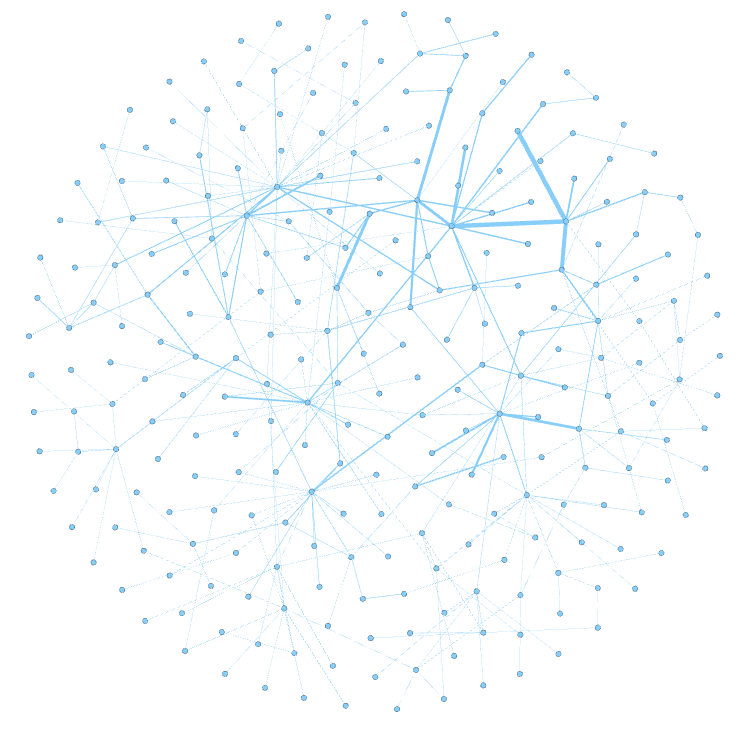
\includegraphics[width=0.5\textwidth]{../visualizacion/q2_fr_spain}
            \label{q2frsp}
        }
        \subfigure[PFNET($r = \infty$, $q = 3$)]{
            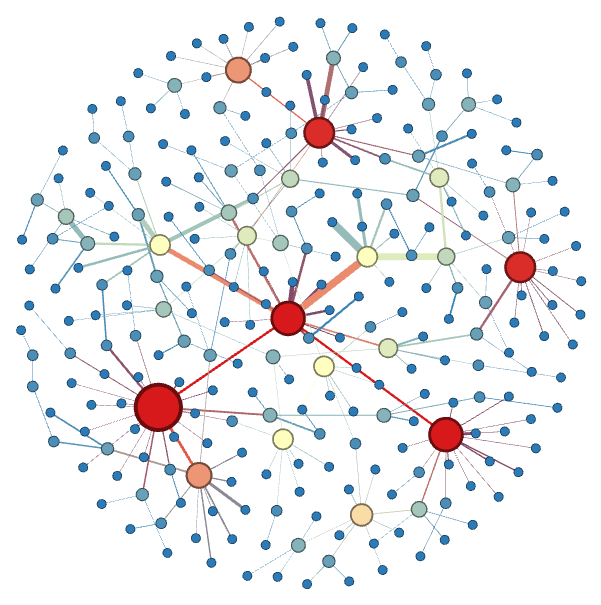
\includegraphics[width=0.5\textwidth]{../visualizacion/q3_fr_spain}
            \label{q3frsp}
        }
    }
    \mbox{
        \subfigure[PFNET($r = \infty$, $q = 4$)]{
            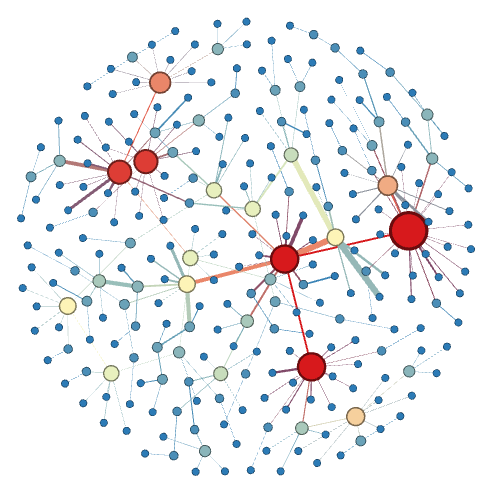
\includegraphics[width=0.5\textwidth]{../visualizacion/q4_fr_spain}
            \label{q4frsp}
        }
        \subfigure[PFNET($r = \infty$, $q = n-1$)]{
            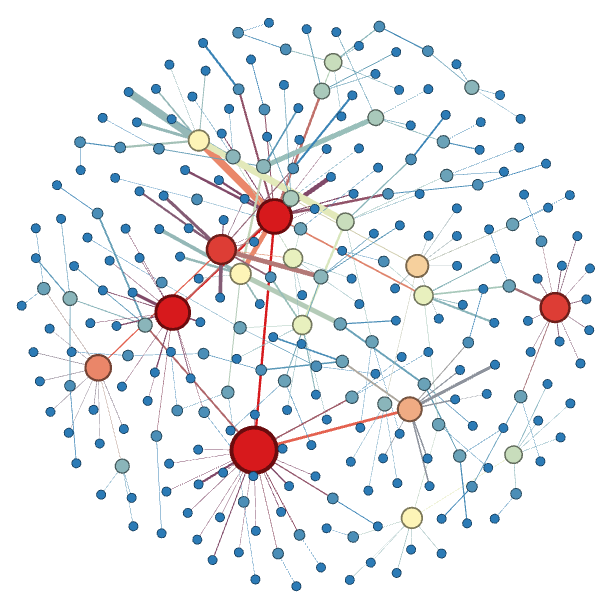
\includegraphics[width=0.5\textwidth]{../visualizacion/qn_fr_spain}
            \label{qnfrsp}
        }
    }
    \caption{Visualizaciones de las PFNETs del cienciograma Spain-2002 realizadas con el método de distribución F-R}
    \label{frsp}
\end{figure}

\begin{figure}[!h]
    \centering
    \mbox{
        \subfigure[PFNET($r = \infty$, $q = 2$)]{
            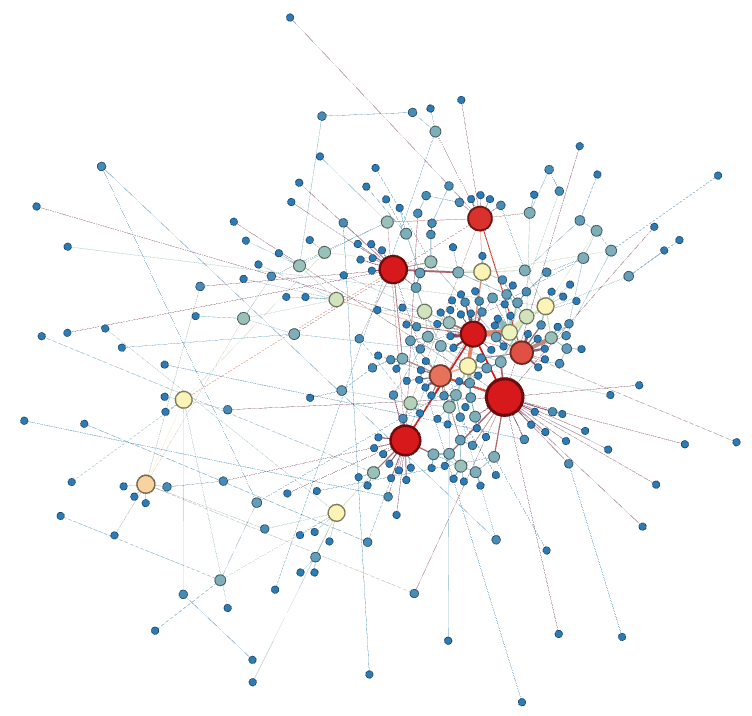
\includegraphics[width=0.5\textwidth]{../visualizacion/q2_kk_spain}
            \label{q2kksp}
        }
        \subfigure[PFNET($r = \infty$, $q = 3$)]{
            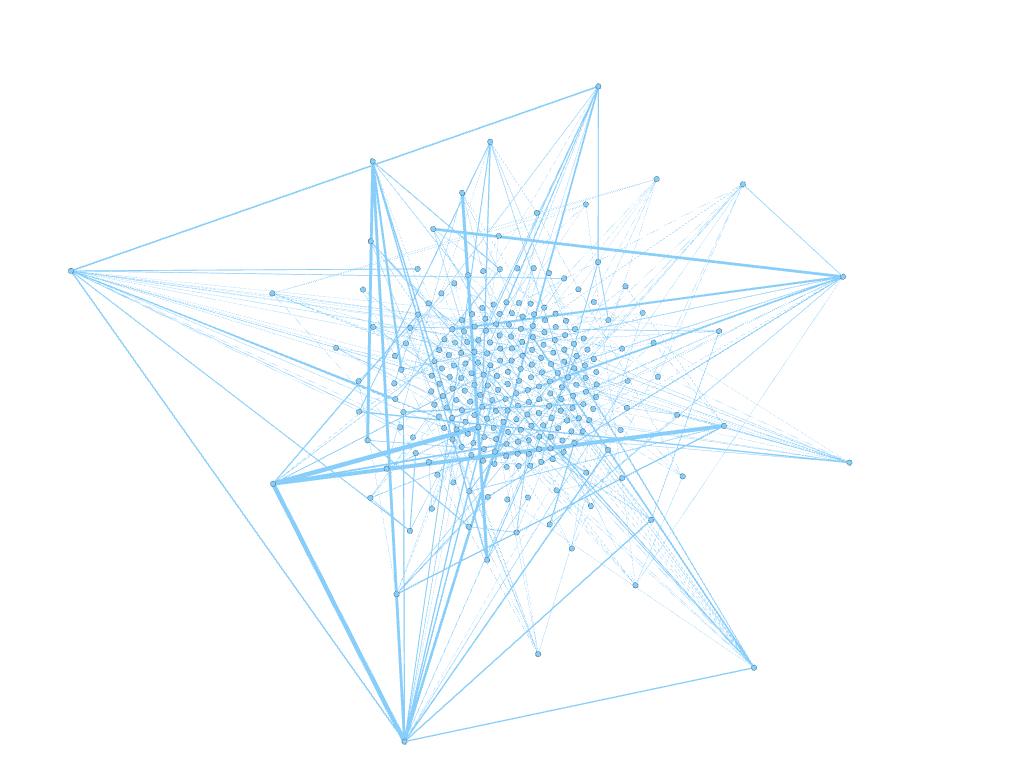
\includegraphics[width=0.5\textwidth]{../visualizacion/q3_kk_spain}
            \label{q3kksp}
        }
    }
    \mbox{
        \subfigure[PFNET($r = \infty$, $q = 4$)]{
            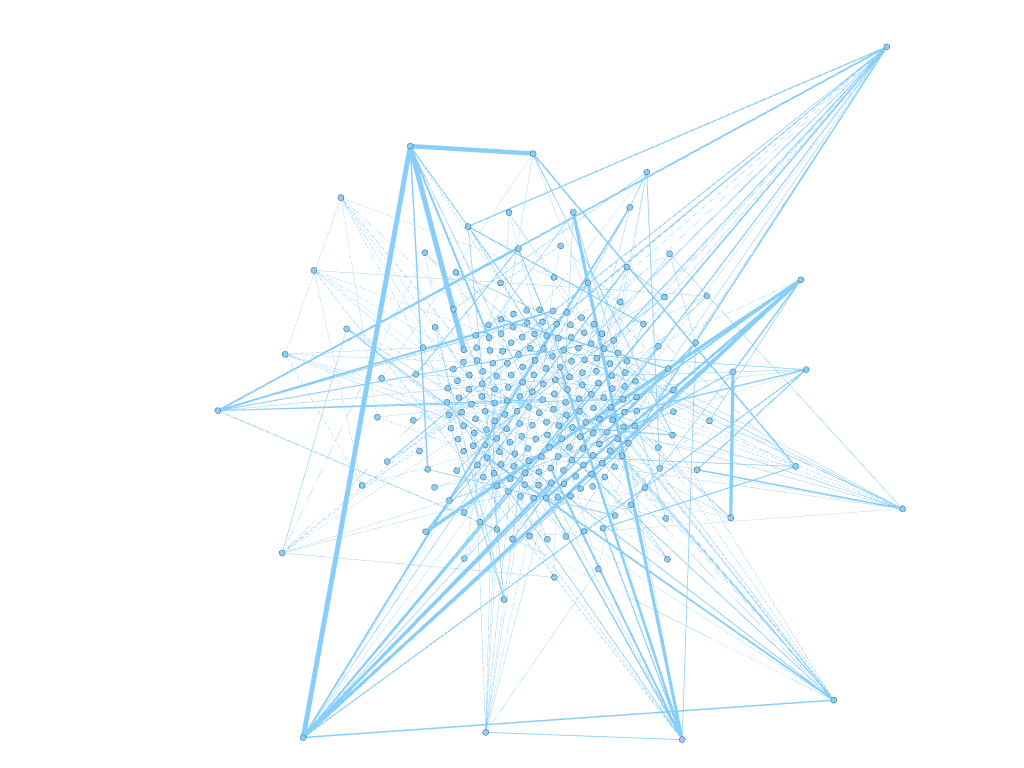
\includegraphics[width=0.5\textwidth]{../visualizacion/q4_kk_spain}
            \label{q4kksp}
        }
        \subfigure[PFNET($r = \infty$, $q = n-1$)]{
            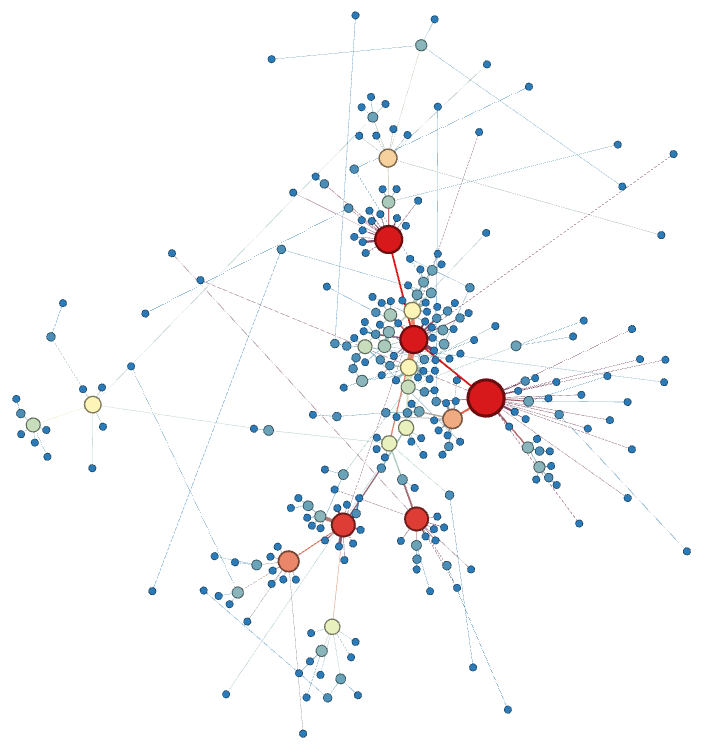
\includegraphics[width=0.5\textwidth]{../visualizacion/qn_kk_spain}
            \label{qnkksp}
        }
    }
    \caption{Visualizaciones de las PFNETs del cienciograma Spain-2002 realizadas con el método de distribución K-K}
    \label{kksp}
\end{figure}

\begin{figure}[!h]
    \centering
    \mbox{
        \subfigure[PFNET($r = \infty$, $q = 2$)]{
            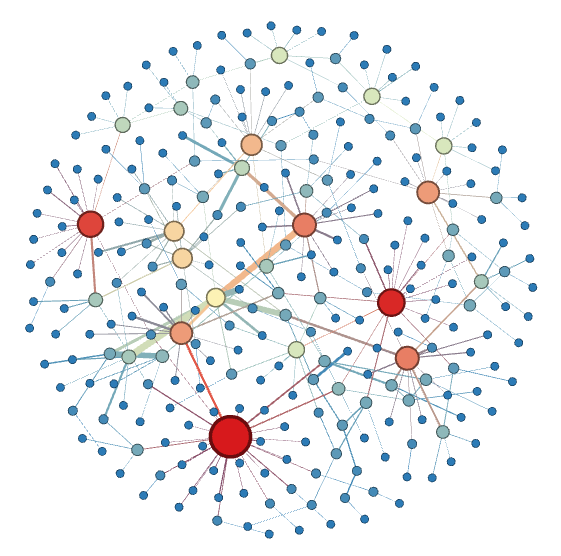
\includegraphics[width=0.5\textwidth]{../visualizacion/q2_fr_us}
            \label{q2frus}
        }
        \subfigure[PFNET($r = \infty$, $q = 3$)]{
            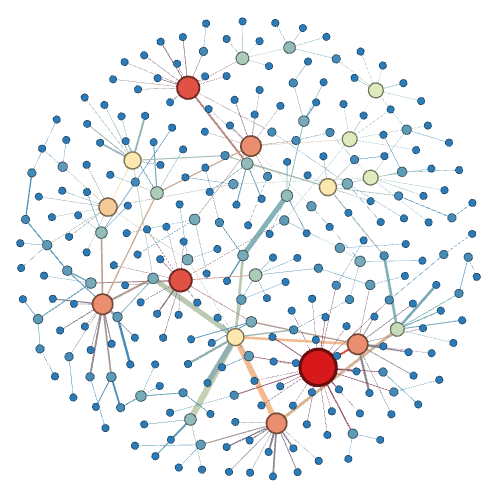
\includegraphics[width=0.5\textwidth]{../visualizacion/q3_fr_us}
            \label{q3frus}
        }
    }
    \mbox{
        \subfigure[PFNET($r = \infty$, $q = 4$)]{
            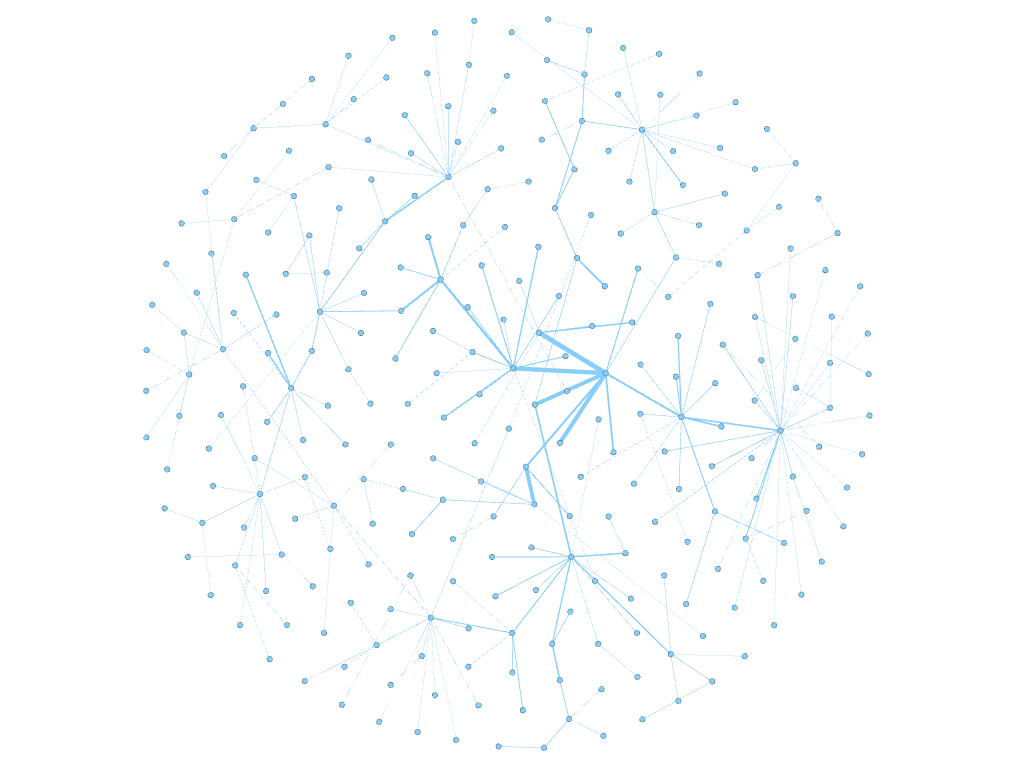
\includegraphics[width=0.5\textwidth]{../visualizacion/q4_fr_us}
            \label{q4frus}
        }
        \subfigure[PFNET($r = \infty$, $q = n-1$)]{
            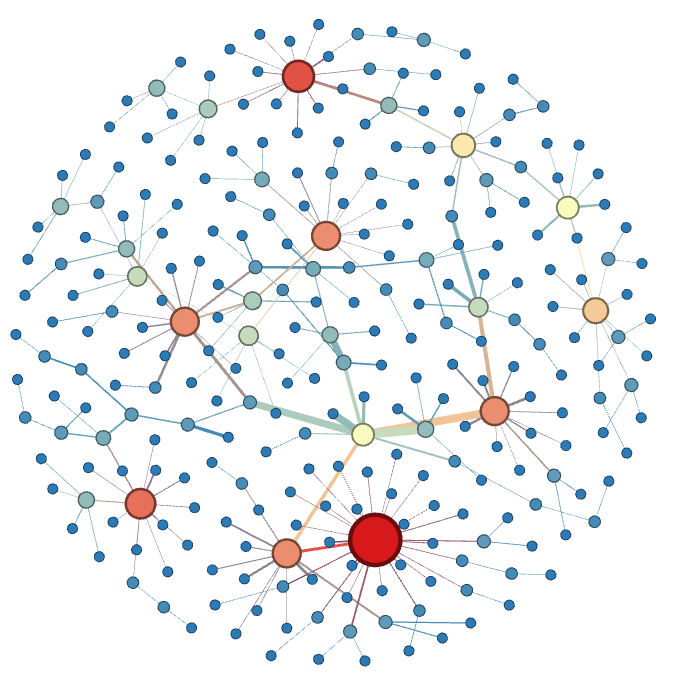
\includegraphics[width=0.5\textwidth]{../visualizacion/qn_fr_us}
            \label{qnfrus}
        }
    }
    \caption{Visualizaciones de las PFNETs del cienciograma United\_States-2002 realizadas con el método de distribución F-R}
    \label{frus}
\end{figure}

\begin{figure}[!h]
    \centering
    \mbox{
        \subfigure[PFNET($r = \infty$, $q = 2$)]{
            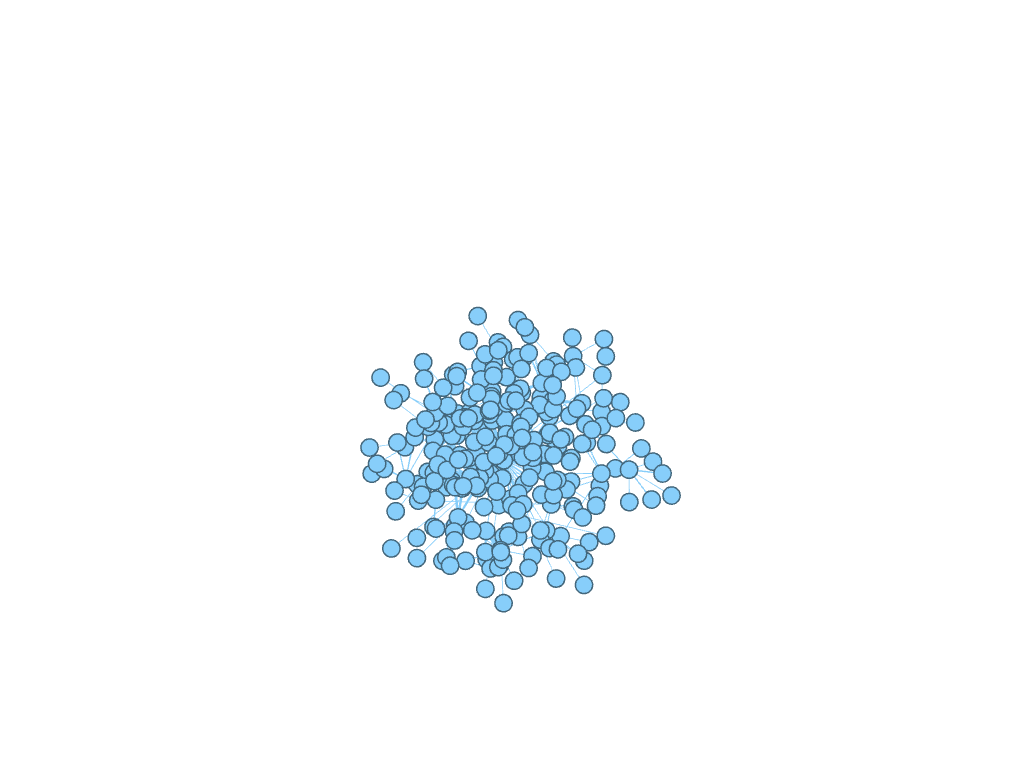
\includegraphics[width=0.5\textwidth]{../visualizacion/q2_kk_us}
            \label{q2kkus}
        }
        \subfigure[PFNET($r = \infty$, $q = 3$)]{
            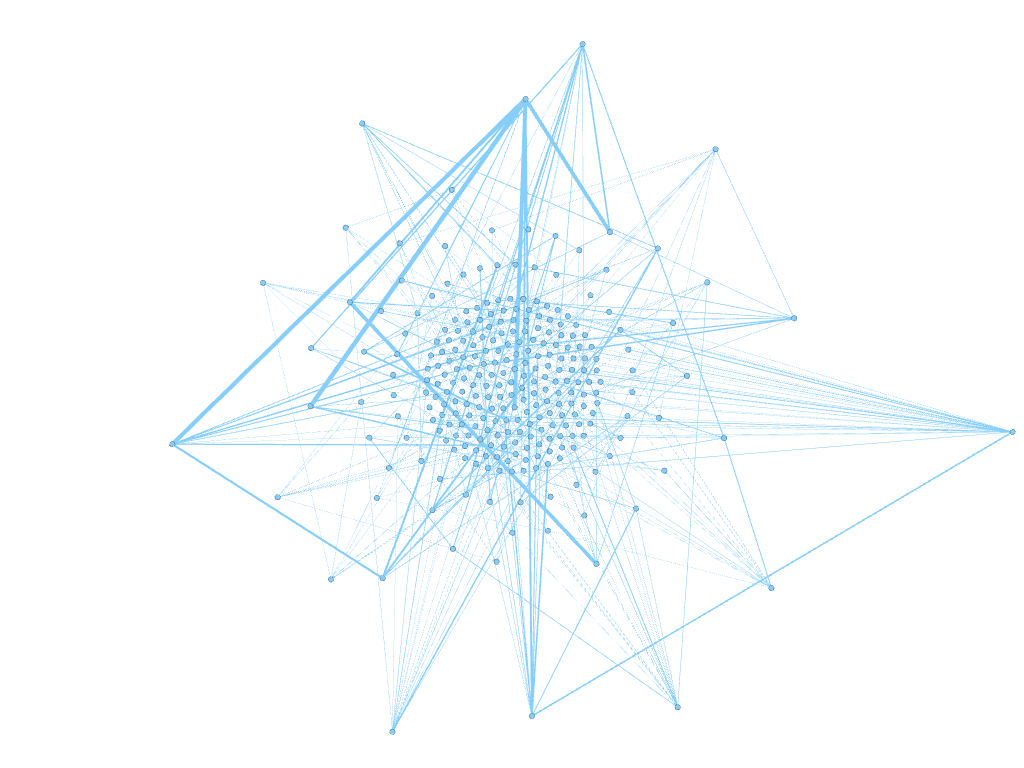
\includegraphics[width=0.5\textwidth]{../visualizacion/q3_kk_us}
            \label{q3kkus}
        }
    }
    \mbox{
        \subfigure[PFNET($r = \infty$, $q = 4$)]{
            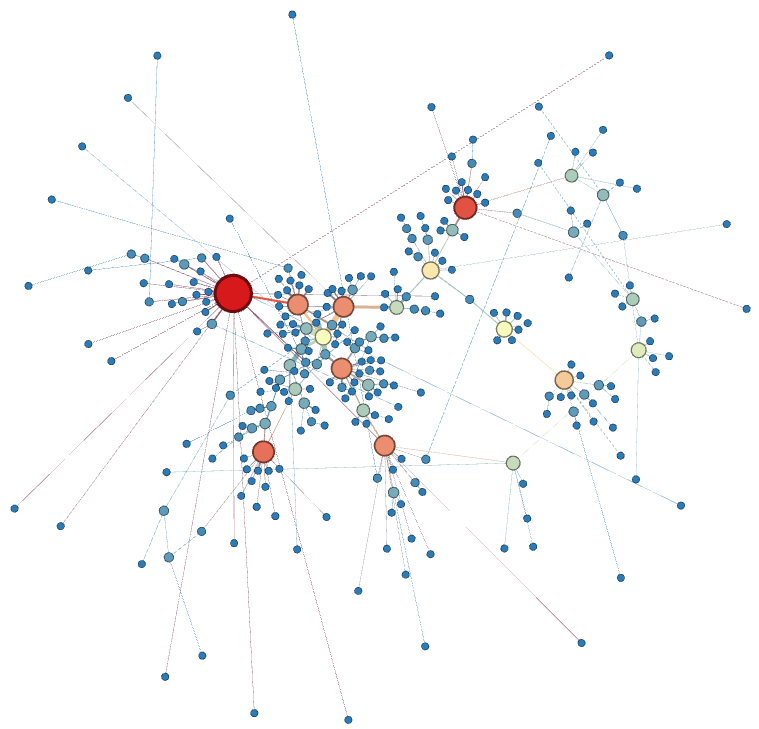
\includegraphics[width=0.5\textwidth]{../visualizacion/q4_kk_us}
            \label{q4kkus}
        }
        \subfigure[PFNET($r = \infty$, $q = n-1$)]{
            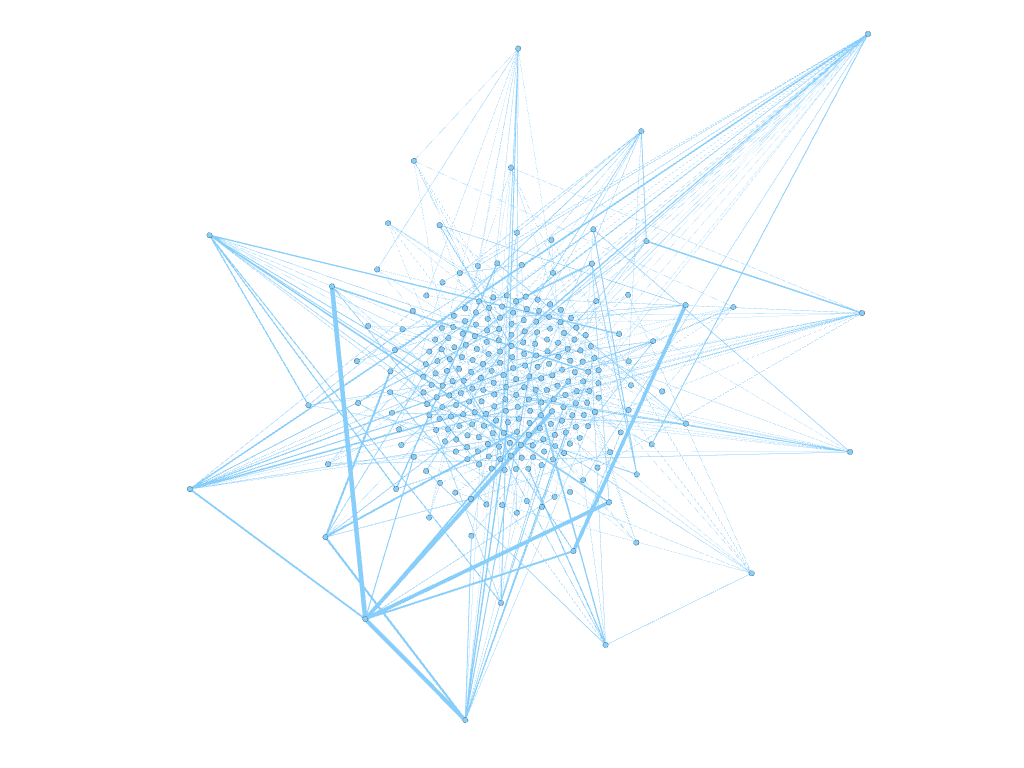
\includegraphics[width=0.5\textwidth]{../visualizacion/qn_kk_us}
            \label{qnkkus}
        }
    }
    \caption{Visualizaciones de las PFNETs del cienciograma United\_States-2002 realizadas con el método de distribución K-K}
    \label{kkus}
\end{figure}

\begin{figure}[!h]
    \centering
    \mbox{
        \subfigure[PFNET($r = \infty$, $q = 2$)]{
            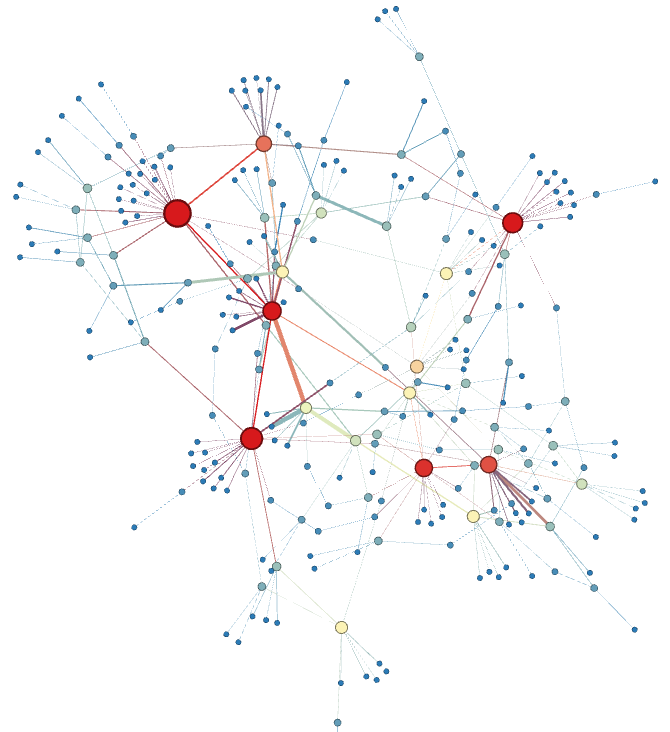
\includegraphics[width=0.5\textwidth]{../visualizacion/q2_yf_sp}
            \label{q2yfsp}
        }
        \subfigure[PFNET($r = \infty$, $q = 3$)]{
            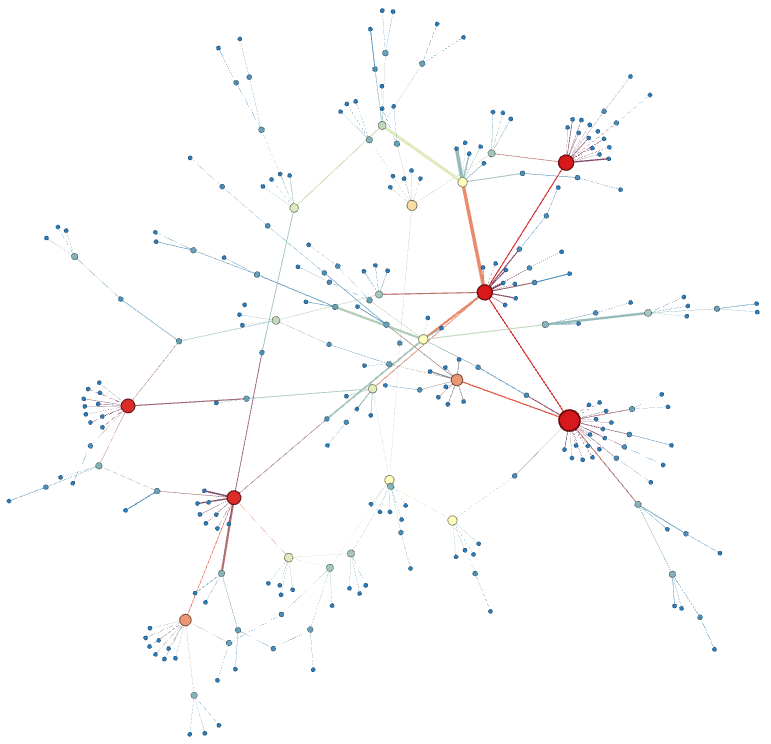
\includegraphics[width=0.5\textwidth]{../visualizacion/q3_yf_sp}
            \label{q3yfsp}
        }
    }
    \mbox{
        \subfigure[PFNET($r = \infty$, $q = 4$)]{
            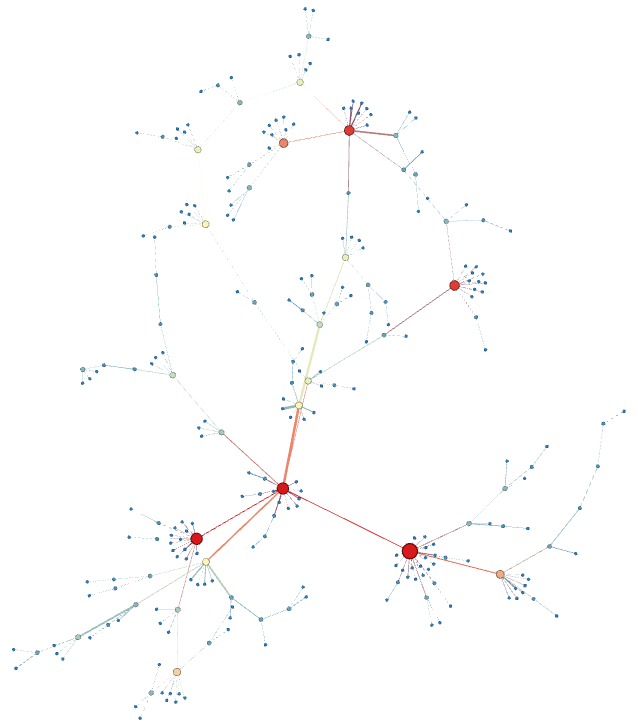
\includegraphics[width=0.5\textwidth]{../visualizacion/q4_yf_sp}
            \label{q4yfsp}
        }
        \subfigure[PFNET($r = \infty$, $q = n-1$)]{
            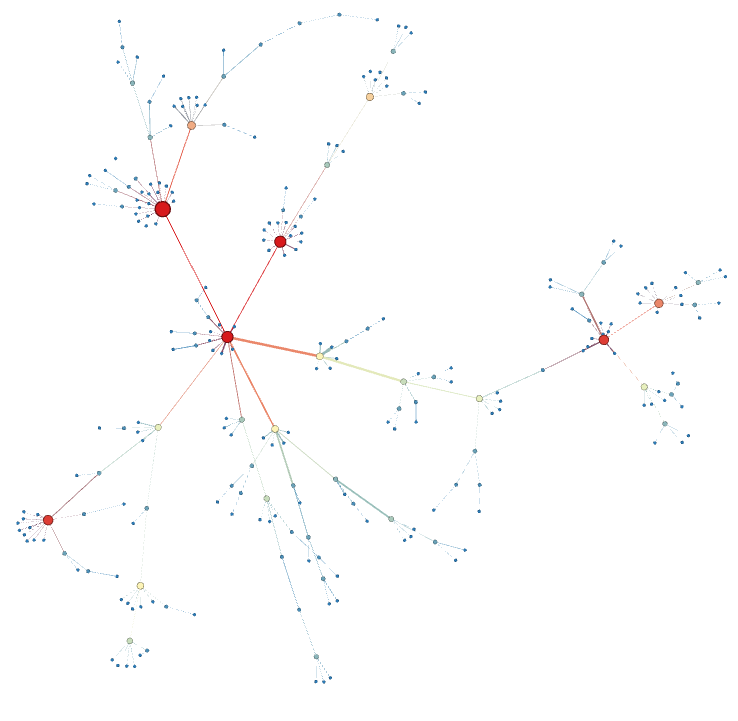
\includegraphics[width=0.5\textwidth]{../visualizacion/qn_yf_sp}
            \label{qnyfsp}
        }
    }
    \caption{Visualizaciones de las PFNETs del cienciograma Spain-2002 realizadas con el método de distribución Yihan-Fu}
    \label{yfsp}
\end{figure}

\begin{figure}[!h]
    \centering
    \mbox{
        \subfigure[PFNET($r = \infty$, $q = 2$)]{
            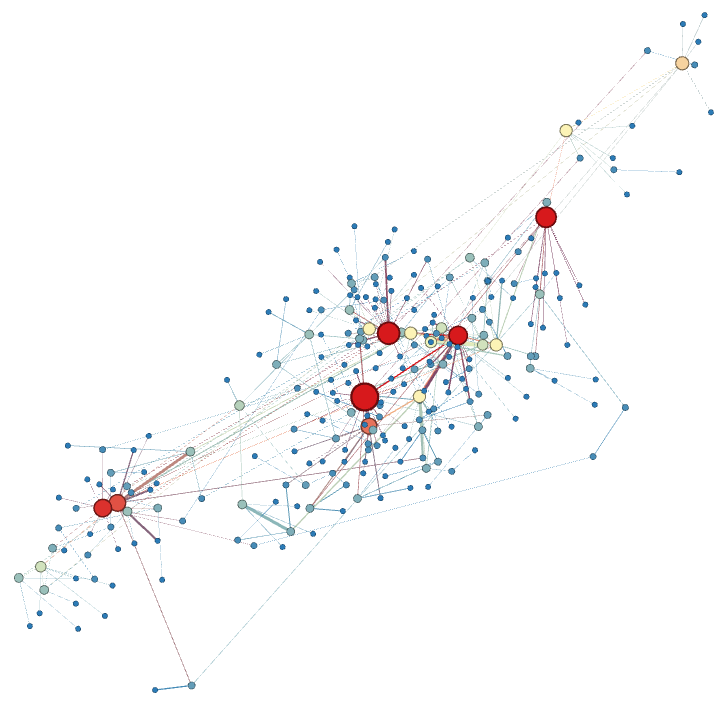
\includegraphics[width=0.5\textwidth]{../visualizacion/q2_oo_sp}
            \label{q2oosp}
        }
        \subfigure[PFNET($r = \infty$, $q = 3$)]{
            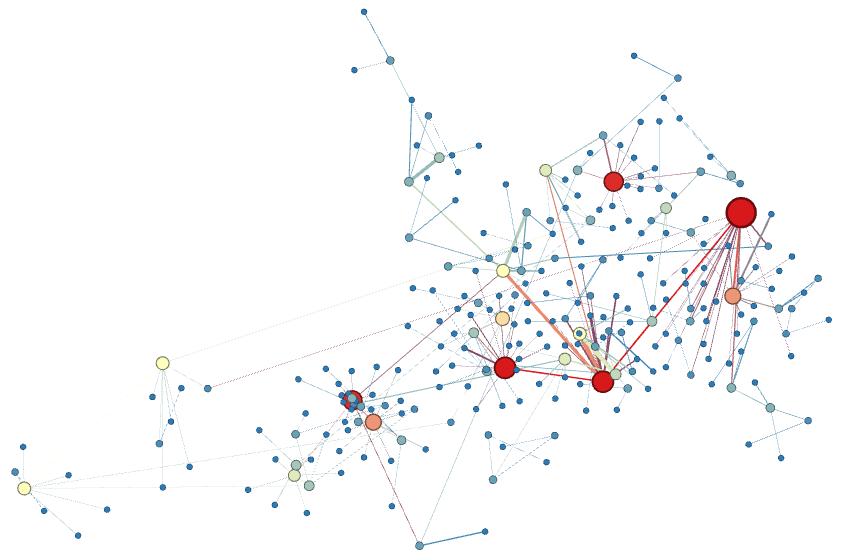
\includegraphics[width=0.5\textwidth]{../visualizacion/q3_oo_sp}
            \label{q3oosp}
        }
    }
    \mbox{
        \subfigure[PFNET($r = \infty$, $q = 4$)]{
            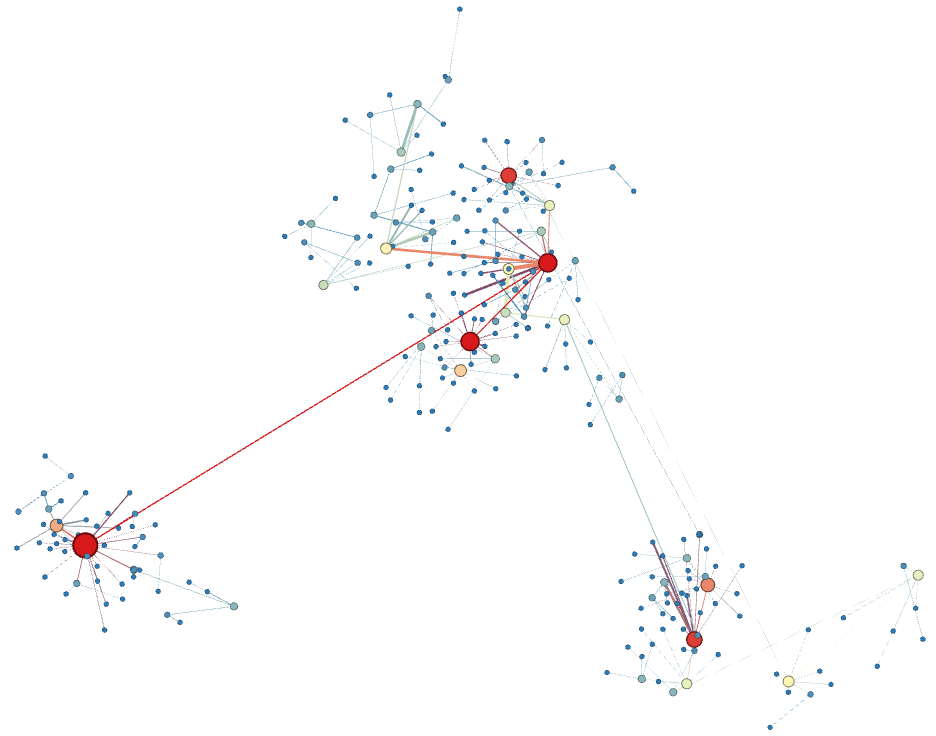
\includegraphics[width=0.5\textwidth]{../visualizacion/q4_oo_sp}
            \label{q4oosp}
        }
        \subfigure[PFNET($r = \infty$, $q = n-1$)]{
            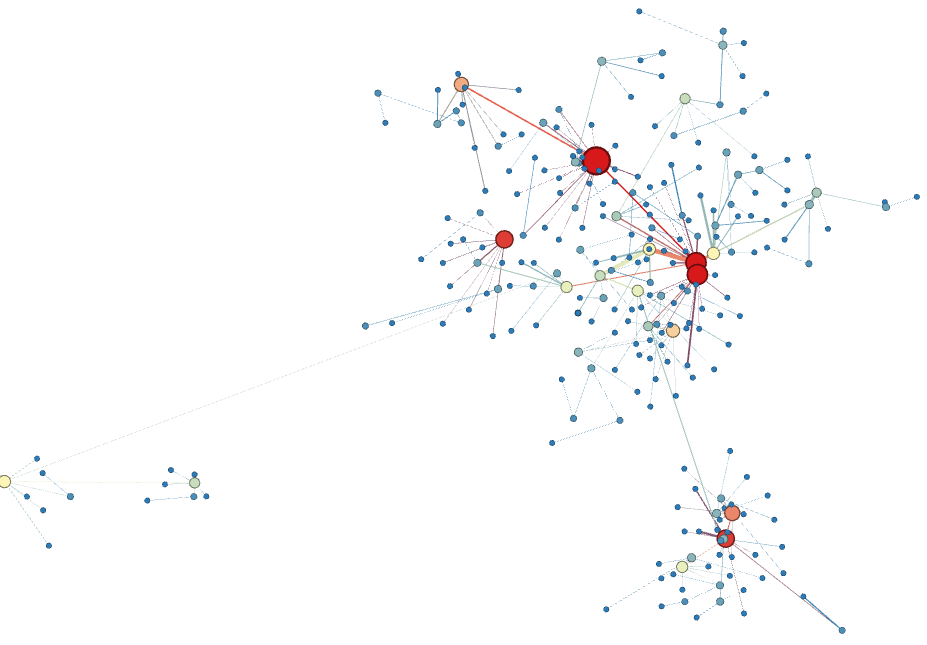
\includegraphics[width=0.5\textwidth]{../visualizacion/qn_oo_sp}
            \label{qnoosp}
        }
    }
    \caption{Visualizaciones de las PFNETs del cienciograma Spain-2002 realizadas con el método de distribución OpenOrd}
    \label{oosp}
\end{figure}

\begin{figure}[!h]
    \centering
    \mbox{
        \subfigure[PFNET($r = \infty$, $q = 2$)]{
            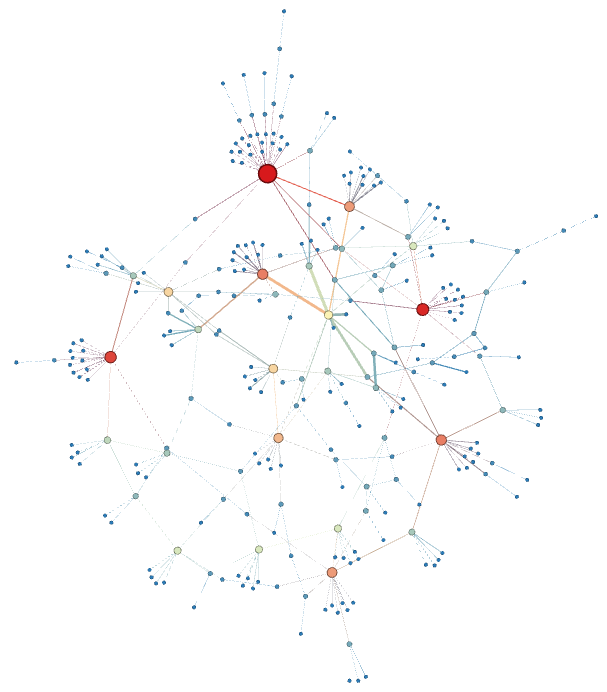
\includegraphics[width=0.5\textwidth]{../visualizacion/q2_yf_us}
            \label{q2yhus}
        }
        \subfigure[PFNET($r = \infty$, $q = 3$)]{
            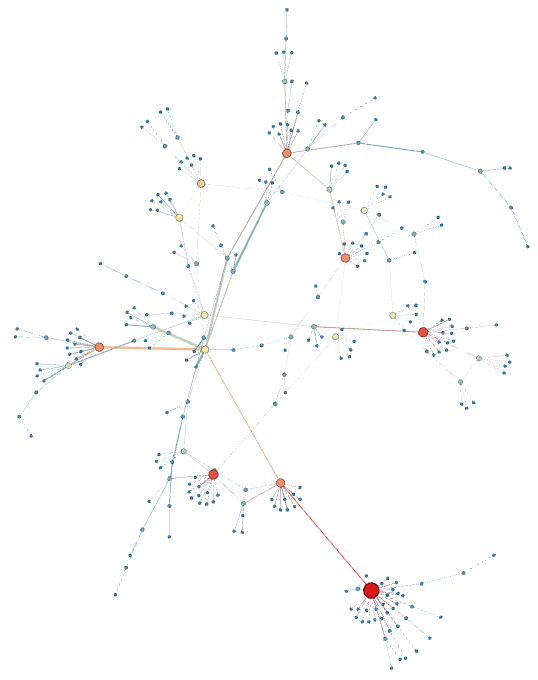
\includegraphics[width=0.5\textwidth]{../visualizacion/q3_yh_us}
            \label{q3yhus}
        }
    }
    \mbox{
        \subfigure[PFNET($r = \infty$, $q = 4$)]{
            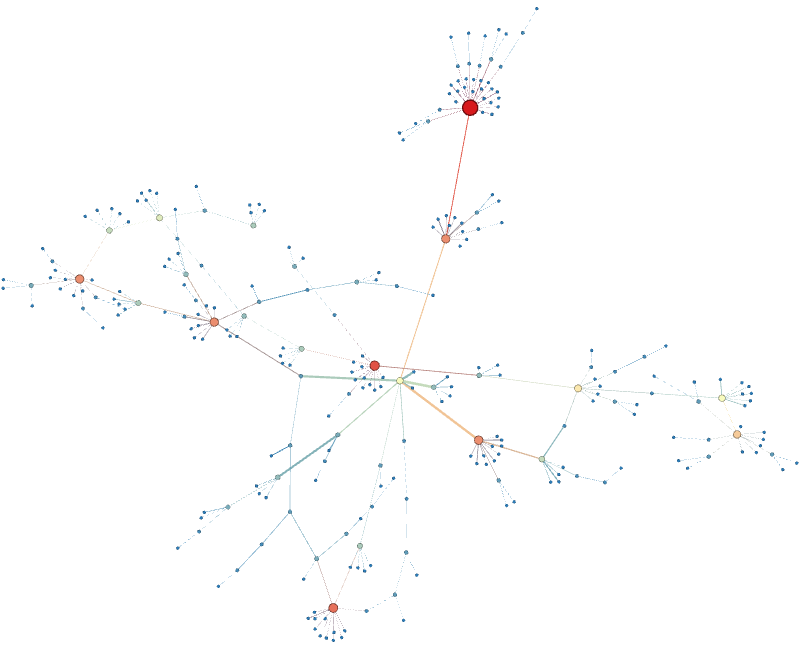
\includegraphics[width=0.5\textwidth]{../visualizacion/q4_yh_us}
            \label{q4yhus}
        }
        \subfigure[PFNET($r = \infty$, $q = n-1$)]{
            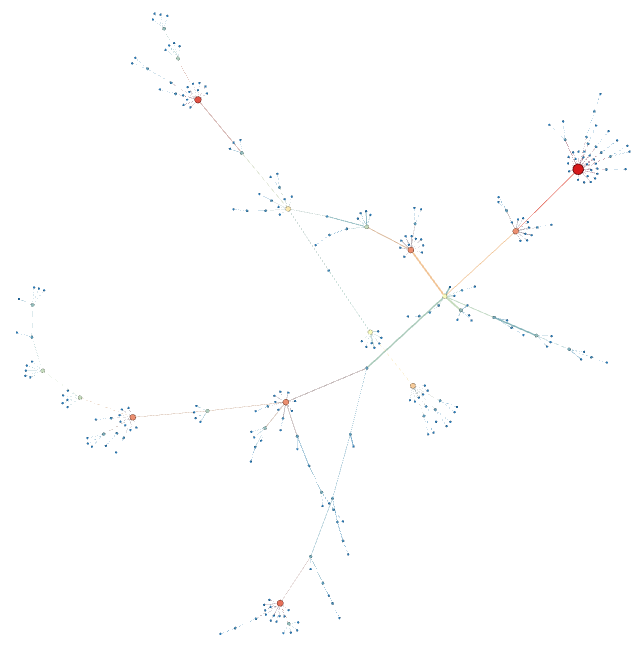
\includegraphics[width=0.5\textwidth]{../visualizacion/qn_yh_us}
            \label{qnyhus}
        }
    }
    \caption{Visualizaciones de las PFNETs del cienciograma United\_States-2002 realizadas con el método de distribución Yihan-Fu}
    \label{yhus}
\end{figure}

\begin{figure}[!h]
    \centering
    \mbox{
        \subfigure[PFNET($r = \infty$, $q = 2$)]{
            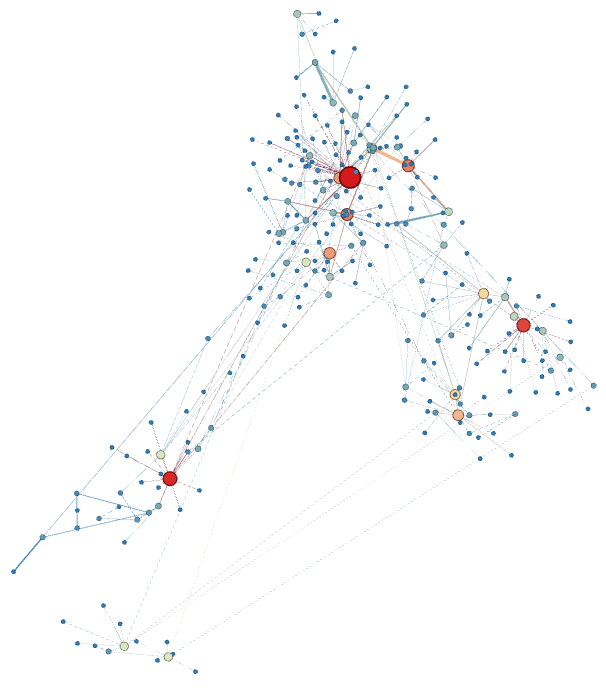
\includegraphics[width=0.5\textwidth]{../visualizacion/q2_oo_us}
            \label{q2oous}
        }
        \subfigure[PFNET($r = \infty$, $q = 3$)]{
            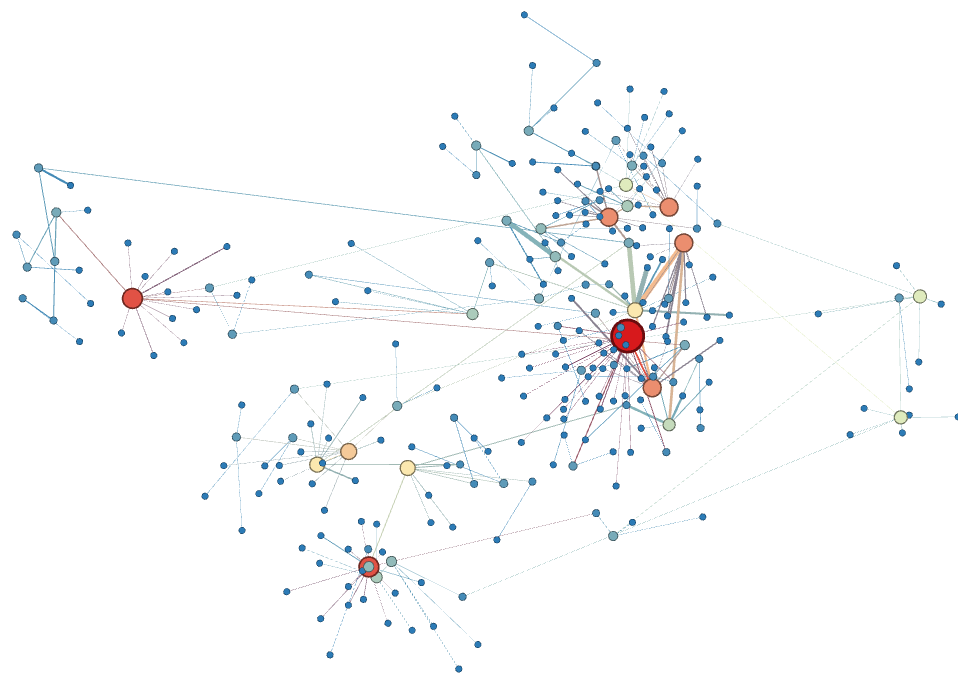
\includegraphics[width=0.5\textwidth]{../visualizacion/q3_oo_us}
            \label{q3oous}
        }
    }
    \mbox{
        \subfigure[PFNET($r = \infty$, $q = 4$)]{
            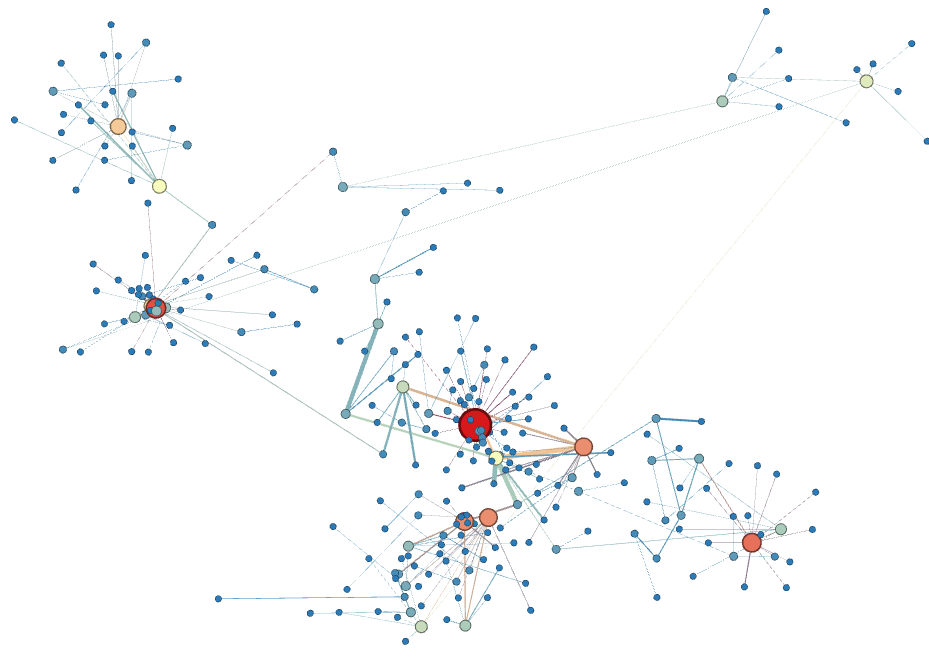
\includegraphics[width=0.5\textwidth]{../visualizacion/q4_oo_us}
            \label{q4oous}
        }
        \subfigure[PFNET($r = \infty$, $q = n-1$)]{
            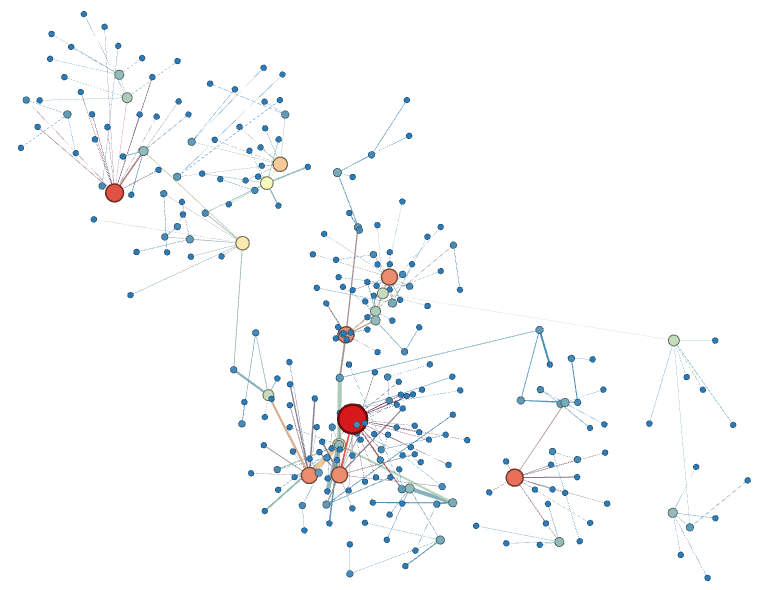
\includegraphics[width=0.5\textwidth]{../visualizacion/qn_oo_us}
            \label{qnoous}
        }
    }
    \caption{Visualizaciones de las PFNETs del cienciograma United\_States-2002 realizadas con el método de distribución OpenOrd}
    \label{oous}
\end{figure}

\begin{figure}[!h]
    \centering
    \mbox{
        \subfigure[PFNET($r = \infty$, $q = 2$)]{
            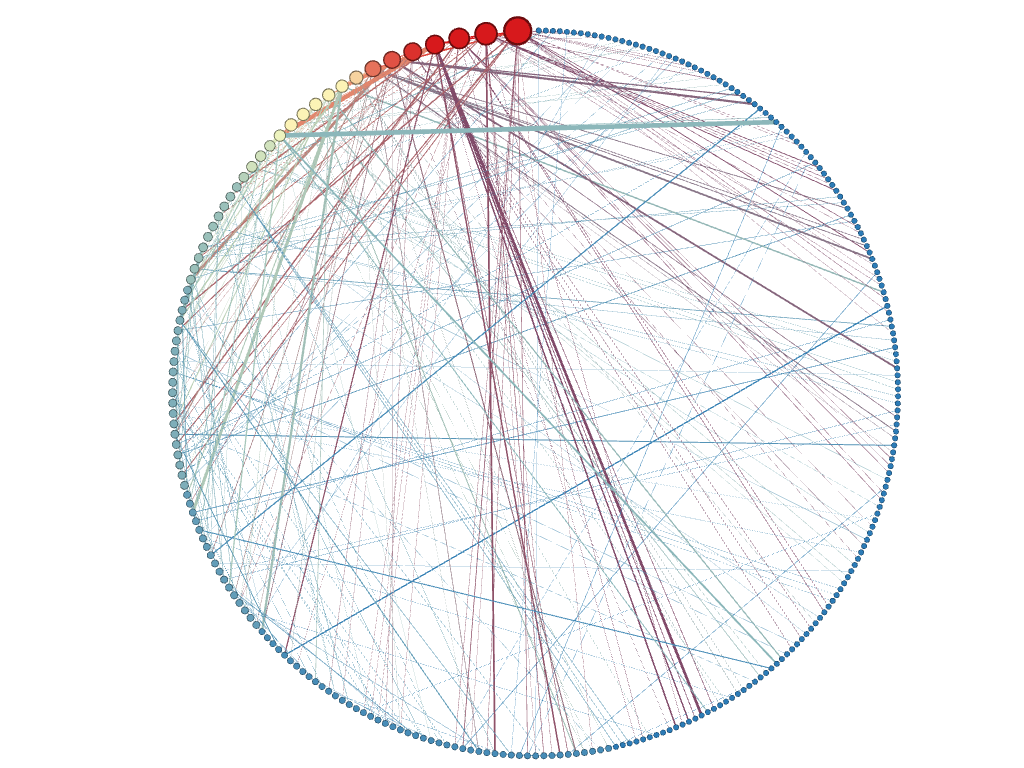
\includegraphics[width=0.5\textwidth]{../visualizacion/q2_cir_sp}
            \label{q2cirsp}
        }
        \subfigure[PFNET($r = \infty$, $q = 3$)]{
            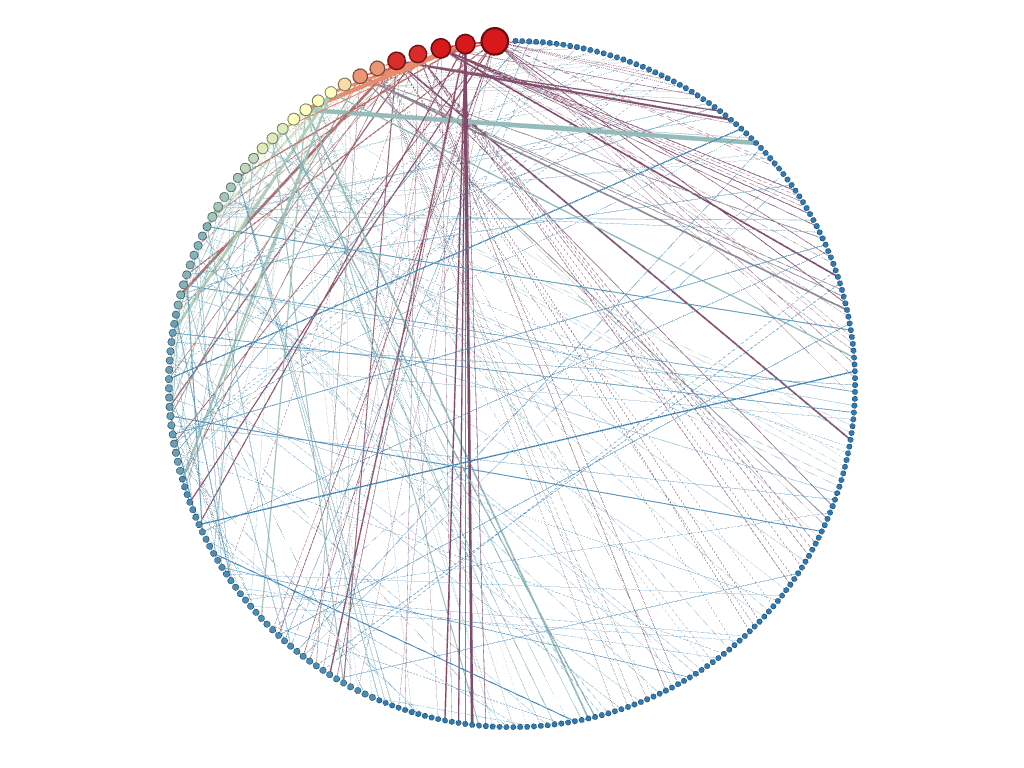
\includegraphics[width=0.5\textwidth]{../visualizacion/q3_cir_sp}
            \label{q3cirsp}
        }
    }
    \mbox{
        \subfigure[PFNET($r = \infty$, $q = 4$)]{
            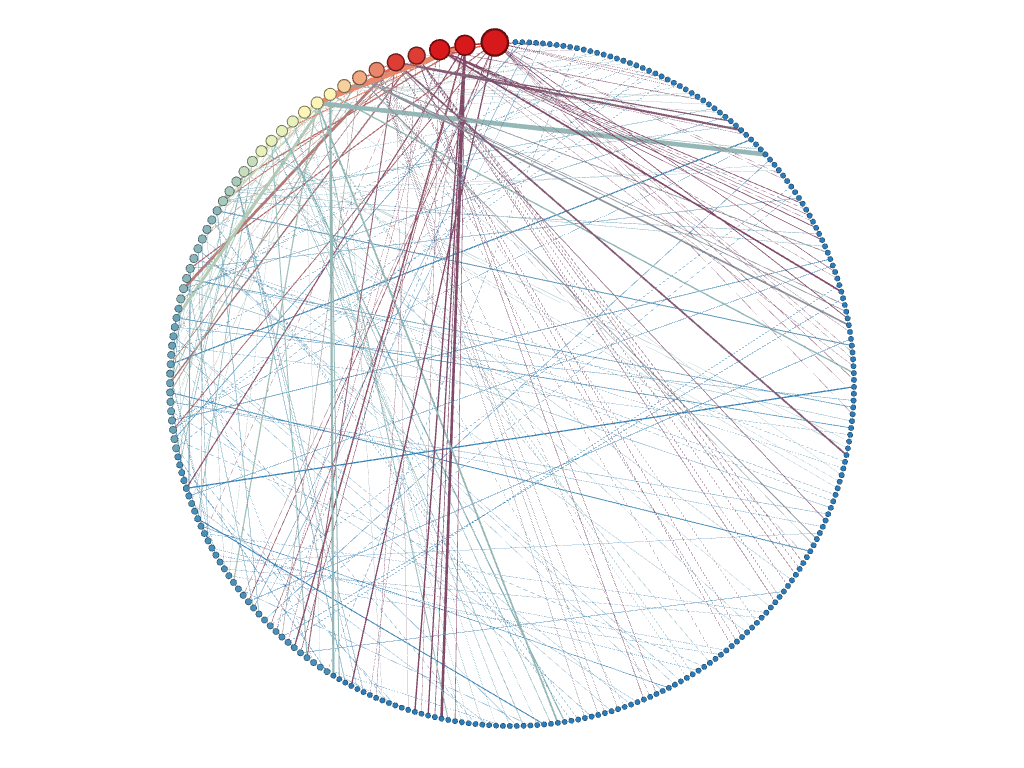
\includegraphics[width=0.5\textwidth]{../visualizacion/q4_cir_sp}
            \label{q4cirsp}
        }
        \subfigure[PFNET($r = \infty$, $q = n-1$)]{
            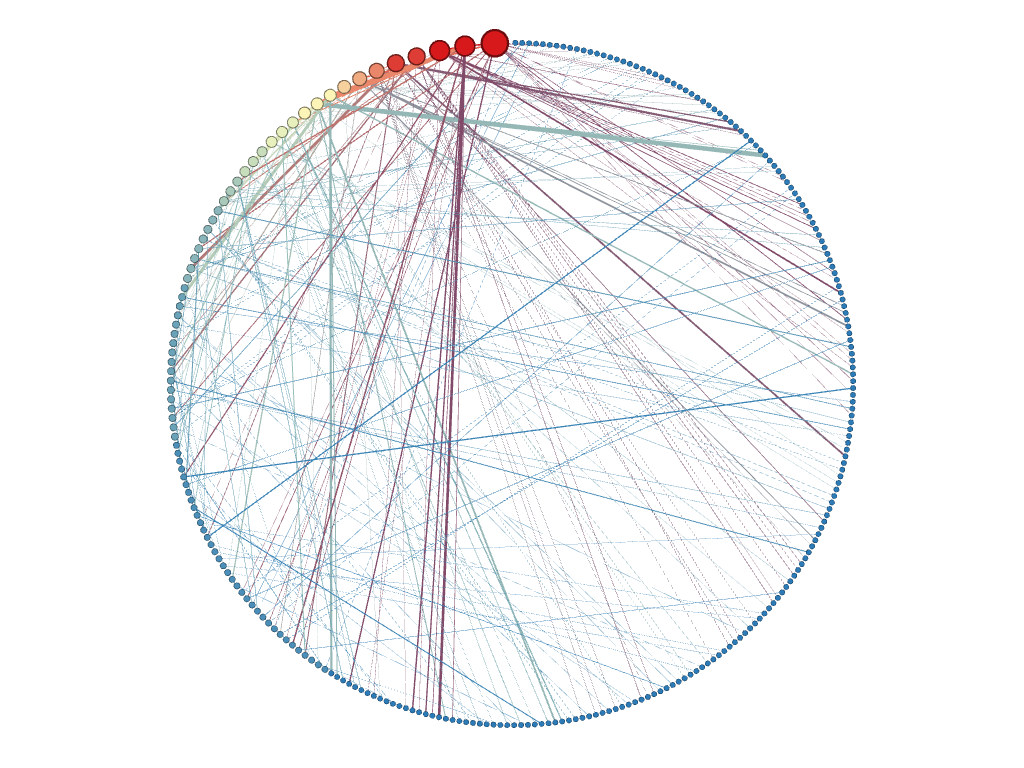
\includegraphics[width=0.5\textwidth]{../visualizacion/qn_cir_sp}
            \label{qncirsp}
        }
    }
    \caption{Visualizaciones de las PFNETs del cienciograma Spain-2002 realizadas con el método de distribución circular}
    \label{cirsp}
\end{figure}

\begin{figure}[!h]
    \centering
    \mbox{
        \subfigure[PFNET($r = \infty$, $q = 2$)]{
            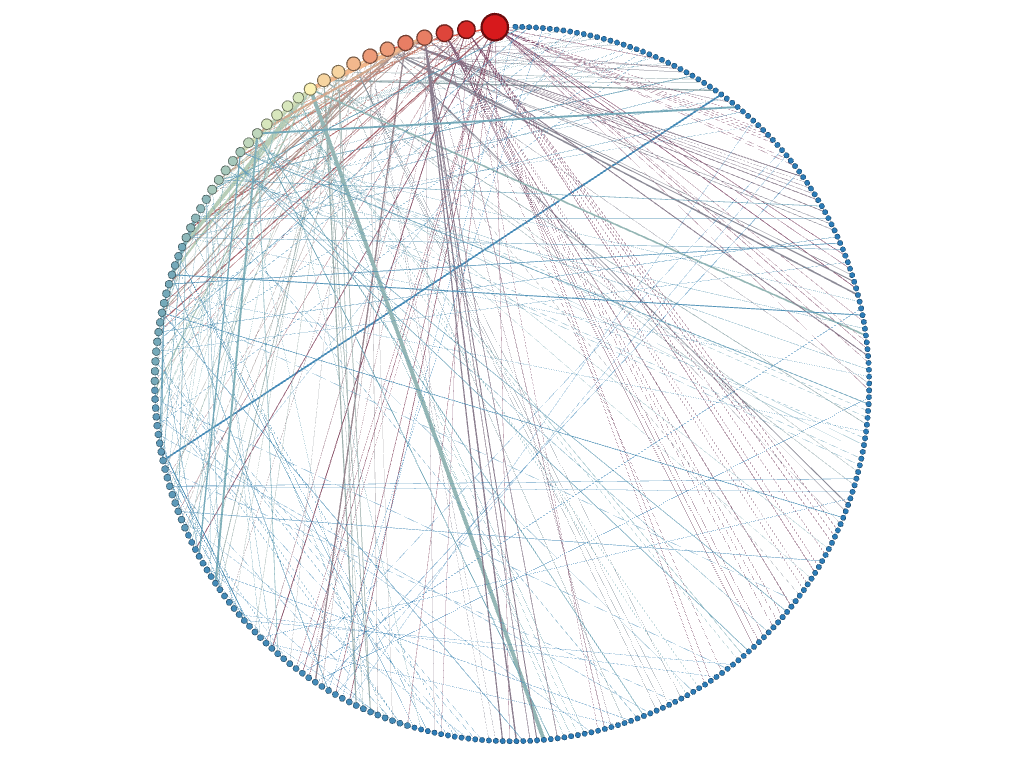
\includegraphics[width=0.5\textwidth]{../visualizacion/q2_cir_us}
            \label{q2cirus}
        }
        \subfigure[PFNET($r = \infty$, $q = 3$)]{
            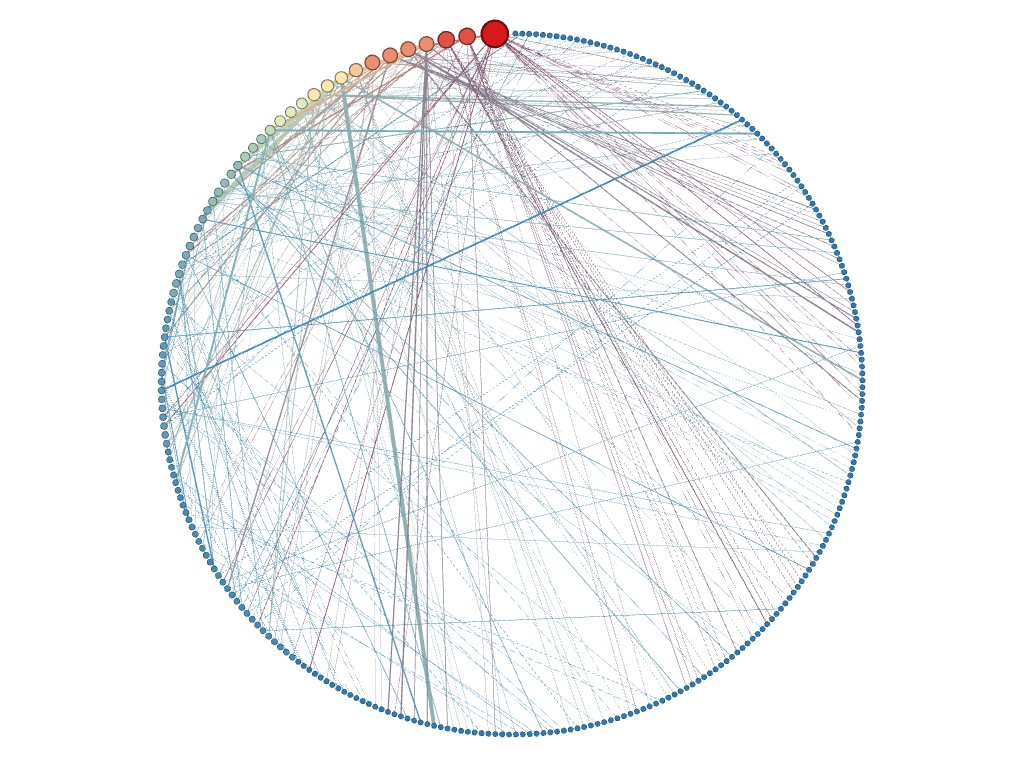
\includegraphics[width=0.5\textwidth]{../visualizacion/q3_cir_us}
            \label{q3cirus}
        }
    }
    \mbox{
        \subfigure[PFNET($r = \infty$, $q = 4$)]{
            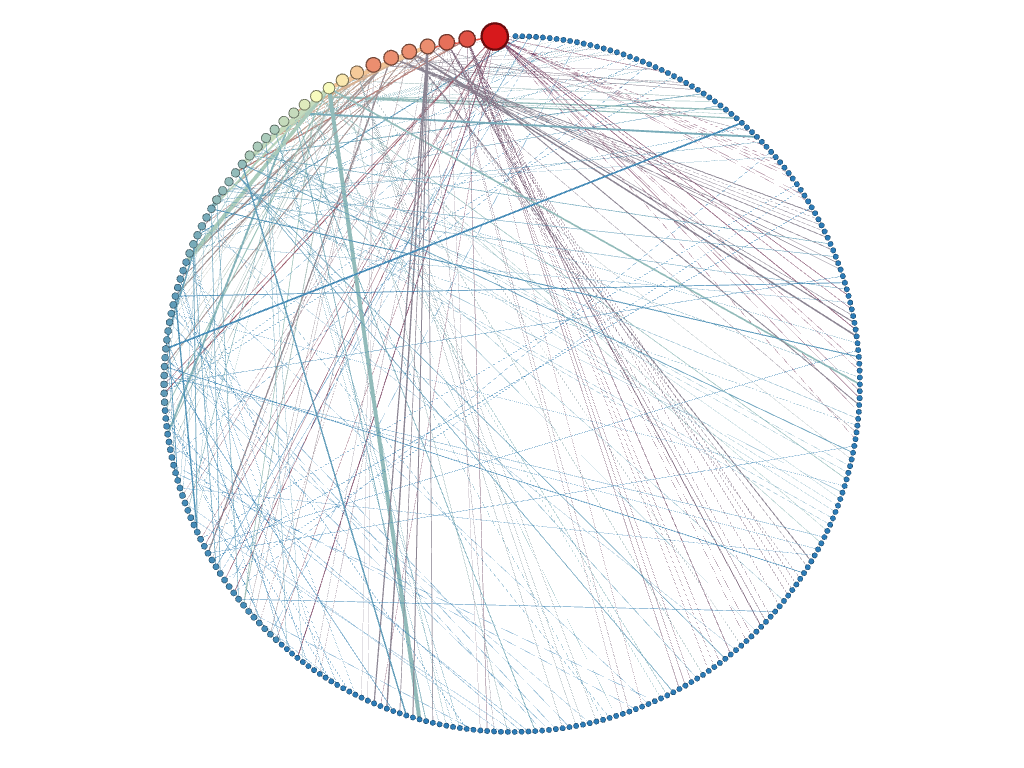
\includegraphics[width=0.5\textwidth]{../visualizacion/q4_cir_us}
            \label{q4cirus}
        }
        \subfigure[PFNET($r = \infty$, $q = n-1$)]{
            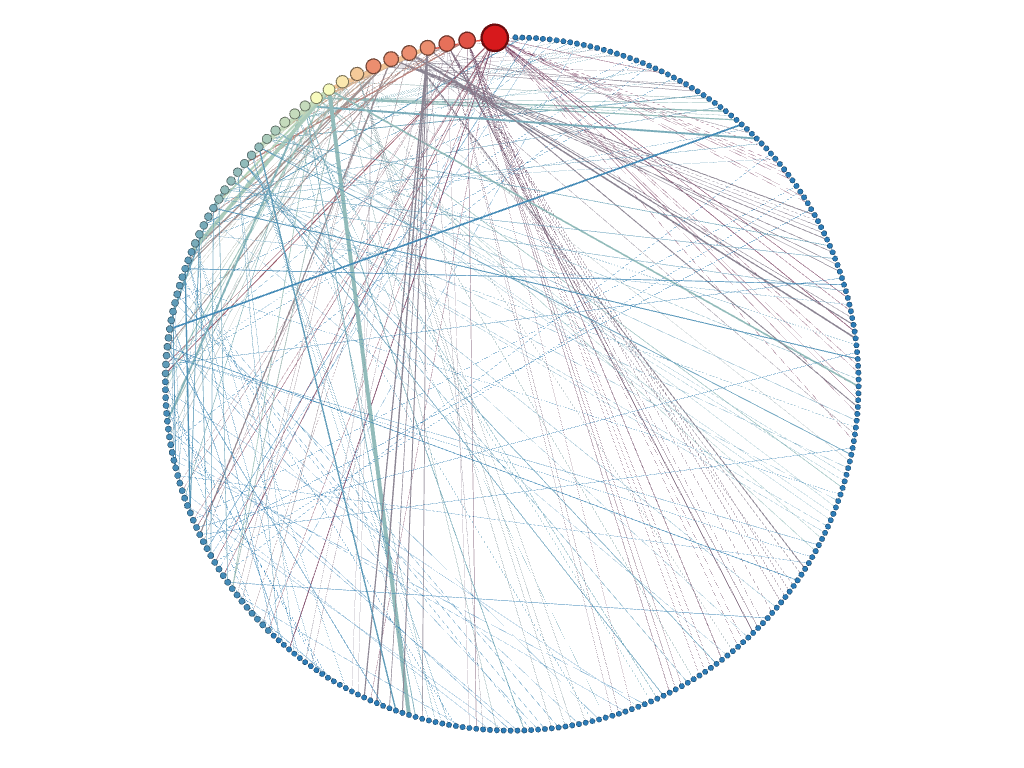
\includegraphics[width=0.5\textwidth]{../visualizacion/qn_cir_us}
            \label{qncirus}
        }
    }
    \caption{Visualizaciones de las PFNETs del cienciograma United\_States-2002 realizadas con el método de distribución circular}
    \label{cirus}
\end{figure}


\section{Análisis de la eficiencia de las distintas variantes de \textit{Pathfinder} en redes de gran tamaño.}
En la \hyperref[tiempopoda]{Tabla \ref*{tiempopoda}} vemos los tiempos obtenidos y la media tanto de enlaces como de densidad para las podas hechas con cada algoritmo. Las redes generadas no eran demasiado densas, en general la densidad media ha sido $D = 0.01$ y el número de enlaces medio está muy por debajo de $L_{max}$ debido a la dispersión de las redes generadas.

En cuanto a los tiempos de ejecución, se ve perfectamente la gran diferencia de tiempo entre el algoritmo \textit{MST} y el resto. Mientras que para el caso más pequeño, 500 nodos, el \textit{original} tarda un minuto y medio, el \textit{MST} tarda menos de un segundo. Esta diferencia se acentúa conforme se aumenta el tamaño de la red: con 10000 nodos, el \textit{original} tarda más de media hora mientras que el \textit{MST}, sólo un segundo. 

No hace falta comparar el algoritmo \textit{original} con el \textit{MST} para encontrarnos un gran salto, éste ya se produce comparándolo con el \textit{Binary}. A pesar de que nos pueda parecer poca la diferencia de eficiencia entre ambos ($O(n^4)$ frente a $O(n^3 log\; n)$) sólo en el caso más pequeño, 500 nodos, el algoritmo \textit{original} es 13 veces más lento. Aún así, en cuanto crece el tamaño de la red a 5000 nodos, el \textit{Binary} queda fuera de juego.

En cuanto al algoritmo \textit{Fast}, consigue una mejora significativa frente al \textit{binary}: $O(n^3 log\; n)$ frente a $O(n^3)$. Esta mejora se hace notar en los tiempos de ejecución: con 2000 nodos, el \textit{binary} es 52 veces más lento que el \textit{fast}. Además, el \textit{fast} experimenta un crecimiento mucho más lento del tiempo de ejecución conforme aumenta la complejidad llegando a aguantar hasta redes con 1000 nodos en un tiempo considerable. 

Por último, tenemos a los \textit{MST} con dos versiones diferentes: ambas difieren en la estructura de datos que utilizan para saber a qué clúster pertenece cada nodo. A pesar de que el algoritmo teórico tiene una mejor eficiencia que el práctico ($O(n^2 log\;n)$ frente a $O(n^3)$) esta pequeña diferencia entre ambos hace que el algoritmo práctico sea más rápido. Esta diferencia es muy pequeña (incluso en redes grandes). De hecho, en la red con 10000 nodos, el algoritmo teórico sólo fue casi dos veces más lento que el práctico. Aún así es una diferencia a tener en cuenta.


% En cuanto a los tiempos de ejecución, vemos cómo encajan con lo que esperábamos. El algoritmo \textit{original} tiene una eficiencia de $O(n^4)$, por lo que en cuanto el número de nodos crece lo más mínimo el tiempo se dispara. Igual pasa con el algoritmo \textit{binary}, pero de forma algo más lenta debido a que su complejidad es $O(n^3 \cdot log n)$. La diferencia de tiempo entre el original y el binario es bastante grande, pero la gran diferencia entre ambos es la eficiencia en espacio. Con el algoritmo \textit{fast}, conseguimos reducir la complejidad hasta $O(n^3)$, lo cual nos permite poder operar con matrices redes algo más grandes pero, como vemos, al llegar a 10000 éste algoritmo también supera el tiempo máximo de ejecución.  Por tanto, vemos como a pesar de que $O(n^3)$ pueda parecer una eficiencia muy buena, en cuanto crece el tamaño de la entrada resulta no ser así.

\begin{table}[!h]
\begin{tabular}{rrrlllll}
\hline
    $N$ &    Media $L$ &   Media $D$ & Original             & Binary               & Fast                 & MST (Teorico)          & MST (Práctico)         \\
\hline
$500$ &   $1252$ & $0.0100$  & $82.9369$  & $6.3309$  & $0.4045$ & $0.0374$ & $0.0065$ \\
$1000$ & $4999$ & $0.0100$   &       $1304.4014$ & $89.3710$  & $2.9496$ & $0.0201$  & $0.0203$ \\
$2000$ &  $20041$ & $0.0100$  &       $> 1800$ & $1234.4935$ & $23.6252$ & $0.1561$  & $0.0792$  \\
$5000$ & $124525$ & $0.0099$ & $> 1800$ & $> 1800$ & $361.3296$   & $0.4194$   & $0.4552$   \\
$10000$ & $498666$ & $0.0099$ & $> 1800$ & $> 1800$ & $> 1800$ & $1.7304$   & $1.5963$    \\
\hline
\end{tabular}
\caption{Tiempos de poda de cada algoritmo}
\label{tiempopoda}
\end{table}

\end{document}

